\documentclass[a4paper]{article}

\usepackage[pdftex,
  hidelinks,
  pdfauthor={Dexter Chua},
  pdfsubject={Cambridge Maths Notes: Part IB - Variational Principles},
  pdftitle={Part IB - Variational Principles},
pdfkeywords={Cambridge Mathematics Maths Math IB Easter Variational Principles}]{hyperref}

\title{Part IB - Variational Principles}
\author{Lectured by P. K. Townsend\\\small Notes taken by Dexter Chua}
\date{Easter 2015}

% Imports
\ifx \nextra \undefined
  \usepackage[pdftex,
    hidelinks,
    pdfauthor={Dexter Chua},
    pdfsubject={Cambridge Maths Notes: Part \npart\ - \ncourse},
    pdftitle={Part \npart\ - \ncourse},
  pdfkeywords={Cambridge Mathematics Maths Math \npart\ \nterm\ \nyear\ \ncourse}]{hyperref}
  \title{Part \npart\ - \ncourse}
\else
  \usepackage[pdftex,
    hidelinks,
    pdfauthor={Dexter Chua},
    pdfsubject={Cambridge Maths Notes: Part \npart\ - \ncourse\ (\nextra)},
    pdftitle={Part \npart\ - \ncourse\ (\nextra)},
  pdfkeywords={Cambridge Mathematics Maths Math \npart\ \nterm\ \nyear\ \ncourse\ \nextra}]{hyperref}

  \title{Part \npart\ - \ncourse \\ {\Large \nextra}}
\fi

\author{Lectured by \nlecturer \\\small Notes taken by Dexter Chua}
\date{\nterm\ \nyear}

\usepackage{alltt}
\usepackage{amsfonts}
\usepackage{amsmath}
\usepackage{amssymb}
\usepackage{amsthm}
\usepackage{booktabs}
\usepackage{caption}
\usepackage{enumitem}
\usepackage{fancyhdr}
\usepackage{graphicx}
\usepackage{mathtools}
\usepackage{microtype}
\usepackage{multirow}
\usepackage{pdflscape}
\usepackage{pgfplots}
\usepackage{siunitx}
\usepackage{tabularx}
\usepackage{tikz}
\usepackage{tkz-euclide}
\usepackage[normalem]{ulem}
\usepackage[all]{xy}

\pgfplotsset{compat=1.12}

\pagestyle{fancyplain}
\lhead{\emph{\nouppercase{\leftmark}}}
\ifx \nextra \undefined
  \rhead{
    \ifnum\thepage=1
    \else
      \npart\ \ncourse
    \fi}
\else
  \rhead{
    \ifnum\thepage=1
    \else
      \npart\ \ncourse\ (\nextra)
    \fi}
\fi
\usetikzlibrary{arrows}
\usetikzlibrary{decorations.markings}
\usetikzlibrary{decorations.pathmorphing}
\usetikzlibrary{positioning}
\usetikzlibrary{fadings}
\usetikzlibrary{intersections}
\usetikzlibrary{cd}

\newcommand*{\Cdot}{\raisebox{-0.25ex}{\scalebox{1.5}{$\cdot$}}}
\newcommand {\pd}[2][ ]{
  \ifx #1 { }
    \frac{\partial}{\partial #2}
  \else
    \frac{\partial^{#1}}{\partial #2^{#1}}
  \fi
}

% Theorems
\theoremstyle{definition}
\newtheorem*{aim}{Aim}
\newtheorem*{axiom}{Axiom}
\newtheorem*{claim}{Claim}
\newtheorem*{cor}{Corollary}
\newtheorem*{defi}{Definition}
\newtheorem*{eg}{Example}
\newtheorem*{fact}{Fact}
\newtheorem*{law}{Law}
\newtheorem*{lemma}{Lemma}
\newtheorem*{notation}{Notation}
\newtheorem*{prop}{Proposition}
\newtheorem*{thm}{Theorem}

\renewcommand{\labelitemi}{--}
\renewcommand{\labelitemii}{$\circ$}
\renewcommand{\labelenumi}{(\roman{*})}

\let\stdsection\section
\renewcommand\section{\newpage\stdsection}

% Strike through
\def\st{\bgroup \ULdepth=-.55ex \ULset}

% Maths symbols
\newcommand{\bra}{\langle}
\newcommand{\ket}{\rangle}

\newcommand{\N}{\mathbb{N}}
\newcommand{\Z}{\mathbb{Z}}
\newcommand{\Q}{\mathbb{Q}}
\renewcommand{\H}{\mathbb{H}}
\newcommand{\R}{\mathbb{R}}
\newcommand{\C}{\mathbb{C}}
\newcommand{\Prob}{\mathbb{P}}
\renewcommand{\P}{\mathbb{P}}
\newcommand{\E}{\mathbb{E}}
\newcommand{\F}{\mathbb{F}}
\newcommand{\cU}{\mathcal{U}}
\newcommand{\RP}{\mathbb{RP}}
\newcommand{\CP}{\mathbb{CP}}

\newcommand{\ph}{\,\cdot\,}

\DeclareMathOperator{\sech}{sech}
\DeclareMathOperator{\cosech}{cosech}
\DeclareMathOperator{\cosec}{cosec}

\DeclareMathOperator{\covol}{covol}
\DeclareMathOperator{\vol}{vol}

\let\Im\relax
\let\Re\relax
\DeclareMathOperator{\Im}{Im}
\DeclareMathOperator{\Re}{Re}
\DeclareMathOperator{\im}{im}
\DeclareMathOperator{\image}{image}
\DeclareMathOperator{\Ann}{Ann}

\DeclareMathOperator*{\res}{res}
\DeclareMathOperator{\Res}{Res}
\DeclareMathOperator{\Ind}{Ind}

\DeclareMathOperator{\tr}{tr}
\DeclareMathOperator{\diag}{diag}
\DeclareMathOperator{\rank}{rank}
\DeclareMathOperator{\card}{card}
\DeclareMathOperator{\spn}{span}
\DeclareMathOperator{\adj}{adj}

\DeclareMathOperator{\erf}{erf}
\DeclareMathOperator{\erfc}{erfc}

\DeclareMathOperator{\ord}{ord}
\DeclareMathOperator{\Sym}{Sym}

\DeclareMathOperator{\sgn}{sgn}
\DeclareMathOperator{\orb}{orb}
\DeclareMathOperator{\stab}{stab}
\DeclareMathOperator{\ccl}{ccl}

\DeclareMathOperator{\lcm}{lcm}
\DeclareMathOperator{\hcf}{hcf}

\DeclareMathOperator{\Int}{Int}
\DeclareMathOperator{\id}{id}

\DeclareMathOperator{\betaD}{beta}
\DeclareMathOperator{\gammaD}{gamma}
\DeclareMathOperator{\Poisson}{Poisson}
\DeclareMathOperator{\binomial}{binomial}
\DeclareMathOperator{\multinomial}{multinomial}
\DeclareMathOperator{\Bernoulli}{Bernoulli}
\DeclareMathOperator{\like}{like}

\DeclareMathOperator{\var}{var}
\DeclareMathOperator{\cov}{cov}
\DeclareMathOperator{\bias}{bias}
\DeclareMathOperator{\mse}{mse}
\DeclareMathOperator{\corr}{corr}

\DeclareMathOperator{\otp}{otp}
\DeclareMathOperator{\dom}{dom}

\DeclareMathOperator{\Root}{Root}
\DeclareMathOperator{\supp}{supp}
\DeclareMathOperator{\rel}{rel}
\DeclareMathOperator{\Hom}{Hom}
\DeclareMathOperator{\Aut}{Aut}
\DeclareMathOperator{\Gal}{Gal}
\DeclareMathOperator{\Mat}{Mat}
\DeclareMathOperator{\End}{End}
\DeclareMathOperator{\Char}{char}
\DeclareMathOperator{\ev}{ev}
\DeclareMathOperator{\St}{St}
\DeclareMathOperator{\Lk}{Lk}
\DeclareMathOperator{\disc}{disc}
\DeclareMathOperator{\Isom}{Isom}
\DeclareMathOperator{\length}{length}
\DeclareMathOperator{\energy}{energy}
\DeclareMathOperator{\area}{area}
\DeclareMathOperator{\Syl}{Syl}
\DeclareMathOperator{\cl}{cl}
\DeclareMathOperator{\fix}{fix}

\newcommand{\GL}{\mathrm{GL}}
\newcommand{\SL}{\mathrm{SL}}
\newcommand{\PGL}{\mathrm{PGL}}
\newcommand{\PSL}{\mathrm{PSL}}
\newcommand{\PSU}{\mathrm{PSU}}
\newcommand{\Or}{\mathrm{O}}
\newcommand{\SO}{\mathrm{SO}}
\newcommand{\U}{\mathrm{U}}
\newcommand{\SU}{\mathrm{SU}}

\renewcommand{\d}{\mathrm{d}}
\newcommand{\D}{\mathrm{D}}

\tikzset{->/.style = {decoration={markings,
                                  mark=at position 1 with {\arrow[scale=2]{latex'}}},
                      postaction={decorate}}}
\tikzset{<-/.style = {decoration={markings,
                                  mark=at position 0 with {\arrowreversed[scale=2]{latex'}}},
                      postaction={decorate}}}
\tikzset{<->/.style = {decoration={markings,
                                   mark=at position 0 with {\arrowreversed[scale=2]{latex'}},
                                   mark=at position 1 with {\arrow[scale=2]{latex'}}},
                       postaction={decorate}}}
\tikzset{->-/.style = {decoration={markings,
                                   mark=at position #1 with {\arrow[scale=2]{latex'}}},
                       postaction={decorate}}}
\tikzset{-<-/.style = {decoration={markings,
                                   mark=at position #1 with {\arrowreversed[scale=2]{latex'}}},
                       postaction={decorate}}}

\tikzset{circ/.style = {fill, circle, inner sep = 0, minimum size = 3}}
\tikzset{mstate/.style={circle, draw, blue, text=black, minimum width=0.7cm}}

\definecolor{mblue}{rgb}{0.2, 0.3, 0.8}
\definecolor{morange}{rgb}{1, 0.5, 0}
\definecolor{mgreen}{rgb}{0.1, 0.4, 0.2}
\definecolor{mred}{rgb}{0.5, 0, 0}

\def\drawcirculararc(#1,#2)(#3,#4)(#5,#6){%
    \pgfmathsetmacro\cA{(#1*#1+#2*#2-#3*#3-#4*#4)/2}%
    \pgfmathsetmacro\cB{(#1*#1+#2*#2-#5*#5-#6*#6)/2}%
    \pgfmathsetmacro\cy{(\cB*(#1-#3)-\cA*(#1-#5))/%
                        ((#2-#6)*(#1-#3)-(#2-#4)*(#1-#5))}%
    \pgfmathsetmacro\cx{(\cA-\cy*(#2-#4))/(#1-#3)}%
    \pgfmathsetmacro\cr{sqrt((#1-\cx)*(#1-\cx)+(#2-\cy)*(#2-\cy))}%
    \pgfmathsetmacro\cA{atan2(#2-\cy,#1-\cx)}%
    \pgfmathsetmacro\cB{atan2(#6-\cy,#5-\cx)}%
    \pgfmathparse{\cB<\cA}%
    \ifnum\pgfmathresult=1
        \pgfmathsetmacro\cB{\cB+360}%
    \fi
    \draw (#1,#2) arc (\cA:\cB:\cr);%
}
\newcommand\getCoord[3]{\newdimen{#1}\newdimen{#2}\pgfextractx{#1}{\pgfpointanchor{#3}{center}}\pgfextracty{#2}{\pgfpointanchor{#3}{center}}}

\def\Xint#1{\mathchoice
   {\XXint\displaystyle\textstyle{#1}}%
   {\XXint\textstyle\scriptstyle{#1}}%
   {\XXint\scriptstyle\scriptscriptstyle{#1}}%
   {\XXint\scriptscriptstyle\scriptscriptstyle{#1}}%
   \!\int}
\def\XXint#1#2#3{{\setbox0=\hbox{$#1{#2#3}{\int}$}
     \vcenter{\hbox{$#2#3$}}\kern-.5\wd0}}
\def\ddashint{\Xint=}
\def\dashint{\Xint-}


\begin{document}
\maketitle
{\small
\noindent Stationary points for functions on $\R^n$. Necessary and sufficient conditions for minima and maxima. Importance of convexity. Variational problems with constraints; method of Lagrange multipliers. The Legendre Transform; need for convexity to ensure invertibility; illustrations from thermodynamics.\hspace*{\fill} [4]

\vspace{5pt}
\noindent The idea of a functional and a functional derivative. First variation for functionals, Euler-Lagrange equations, for both ordinary and partial differential equations. Use of Lagrange multipliers and multiplier functions.\hspace*{\fill} [3]

\vspace{5pt}
\noindent Fermat's principle; geodesics; least action principles, Lagrange's and Hamilton's equations for particles and fields. Noether theorems and first integrals, including two forms of Noether's theorem for ordinary differential equations (energy and momentum, for example). Interpretation in terms of conservation laws.\hspace*{\fill} [3]

\vspace{5pt}
\noindent Second variation for functionals; associated eigenvalue problem.\hspace*{\fill} [2]}

\tableofcontents
\setcounter{section}{-1}
\section{Introduction}
What is variational principles?

We start with a simple example.
\begin{center}
  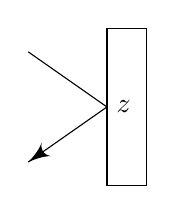
\begin{tikzpicture}
    \draw (1, 1) rectangle (1.5, -1);
    \node at (1, 0) [right] {$z$};
    \draw [->] (0, 0.7) -- (1, 0) -- (0, -0.7);
  \end{tikzpicture}
\end{center}
We see that the light ray travels towards the mirror, gets reflected at $z$, and hits the (invisible) eye. What determines the path? ie. the point $z$ on the mirror? This was answered by Alexandra - the light takes the shortest path. This is a principle, and we use this principle to derive the answer. For example, if $L(z)$ is the length of the path, as a function of $z$, we can solve for $z$ by setting $L'(z) = 0$.

This sounds reasonable - in the absence of mirrors, light travels in a straight line - which is the shortest path between two points.

But is this true? No! Not always. We only considered a plane mirror, and this doesn't hold in we have, say, a spherical mirror. However, it turns out that in all cases, $L'(z) = 0$.

If light travels at finite speed, then the shortest path is the path that gives the minimum time. This is Fermat's principle:
\begin{center}
  Light travels on path that takes the shortest time.
\end{center}
This applies to refraction as well - light rays change direction when travelling between different mediums because they have different speeds in different mediums.

We usually define the refractive index $n$ of a medium to be $n = 1/v$, where $v$ is the velocity of light in the medium. Then we can write the variational principle as
\begin{center}
  maximize $\displaystyle \int_{\text{path}} n\;\d s$,
\end{center}
where $\d s$ is the path length element. This is easy if we have two distinct mediums as above. If $n$ is continuously varying, we need new maths tools - calculus of variations. 

Consider a different problem - Dido's problem. We want to enclose as much area as we wish using a strip of length $L$. We cannot solve this using ordinary calculus. We have an infinite number of paths to try!

We can approximate this by having $n$ pegs on the strip, producing a $n$-gon, and try to maximize it. Then we take $n\to \infty$ and solve our original problem!

\section{Calculus for functions of many variables}
Let $f: \R^n \to \R$ with $\mathbf{x} \mapsto f(\mathbf{x})$. We write $\mathbf{x} = (x_1, \cdots, x_n)$. We assume that $f$ is sufficiently smooth ($C^2(\R)$, ie. twice differentiable, is usually sufficient).  
\begin{defi}[Stationary points]
  \emph{Stationary points} are points in $\R^n$ for which $\nabla f = 0$, ie.
  \[
    \frac{\partial f}{\partial x_1} = \frac{\partial f}{\partial x_2} = \cdots = \frac{\partial f}{\partial x_n} = 0
  \]
\end{defi}
These are not necessarily maximum/minimum. So we expand $f$ in Taylor series about a stationary point $\mathbf{x} = \mathbf{a}$:
\begin{align*}
  f(\mathbf{x}) &= f(\mathbf{a}) + (x - a)\cdot \nabla f + \frac{1}{2}\sum_{i, j}(x_i - a_i)(x_j - a_j)\frac{\partial^2 f}{\partial x_i \partial x_j} + O(x^3).\\
  &= f(\mathbf{a}) + \frac{1}{2}\sum_{i, j}(x_i - a_i)(x_j - a_j)\frac{\partial^2 f}{\partial x_i \partial x_j} + O(x^3).
\end{align*}
The second term is so important that we have a name for it:
\begin{defi}[Hessian matrix]
  The \emph{Hessian matrix} is
  \[
    H_{ij}(x) = \frac{\partial^2 f}{\partial x_i \partial x_j}
  \]
\end{defi}
Of course, we are lazy and choose coordinates such that $\mathbf{a} = \mathbf{0}$. Then
\[
  f(\mathbf{x}) - f(\mathbf{0}) = \frac{1}{2}x_i H_{ij}x_j + O(x^3),
\]
using the summation convention. Since $H$ is symmetric, by rotation of axes, we can diagonalize the quadratic form. Then
\[
  \frac{1}{2}x_i H_{ij}x_j = \frac{1}{2}x_i' H_{ij}'x_j'
\]
with
\[
  H_{ij}' = 
  \begin{pmatrix}
    \lambda_1 & 0 & \cdots & 0\\
    0 & \lambda_2 & \cdots & 0\\
    \vdots & \vdots & \ddots & 0\\
    0 & 0 & \cdots & \lambda_n
  \end{pmatrix}
\]
Since $H$ is symmetric real, the eigenvalues $\lambda_i$ are all symmetric real. Then
\[
  f(\mathbf{x}) - f(\mathbf{0}) = \frac{1}{2}\sum_{i = 0}^n \lambda_i (x_i')^2
\]
Note that this is $\geq 0$ if $\lambda_i > 0$ for all $i$. In this case, stationary point is a local minimum. Similarly, if $\lambda_i < 0$ for all $i$, it is a local minimum. If the eigenvalues have mixed sign, then we go up in some directions, down in others. So we have a saddle point.

If some $\lambda = 0$, we have a \emph{degenerate stationary point}. Here we are in deep, \emph{deep} trouble and have to look at higher derivatives.

\begin{eg}
  Take the boring case where $n = 2$. Then $\det H = \lambda_1, \lambda_2$ and $\tr H = \lambda_1 + \lambda_2$. If $\det H > 0$, then both eigenvalues have same sign. If $\tr H > 0$, both are positive and it is a local minimum. If $\tr H < 0$, it is a local maximum.

  If $\det H < 0$, then the eigenvalues have mixed sign, and it is a saddle. if $\det H = 0$, then it is degenerate.

  For example, let $f(x, y) = x^3 + y^3 - 3xy$. Then
  \[
    \nabla f = 3(x^2 - y, y^2 - x).
  \]
  This is zero iff $x^2 = y$ and $y^2 = x$. So $y^4 = y$. Either $y = 0$, or $y^3 = 1$, ie. $y = 1$. So there are two stationary points: $(0, 0)$ and $(1, 1)$.

  The Hessian matrix is
  \[
    H = 
    \begin{pmatrix}
      6x & -3\\
      -3 & 6y
    \end{pmatrix}
  \]
  So
  \begin{align*}
    \det H &= 9(4xy - 1) = \lambda_1\lambda_2\\
    \tr H &= 6(x + y) = \lambda_1 + \lambda_2
  \end{align*}
  At $(1, 1)$, $\det H > 0$, $\tr H > 0$. So this is a local minimum. At $(0, 0)$, $\det H < 0$. So this is a saddle point.
\end{eg}
\subsection{Convex functions}
\begin{defi}[Convex set]
  A set $S\subseteq \R^n$ is \emph{convex} if for any distinct $\mathbf{x}, \mathbf{y}\in X, t\in (0, 1)$, we have $(1 - t)\mathbf{x} + t\mathbf{y} \in S$. Alternatively, any line joining two points in $S$ lies completely within $S$.

  \begin{center}
    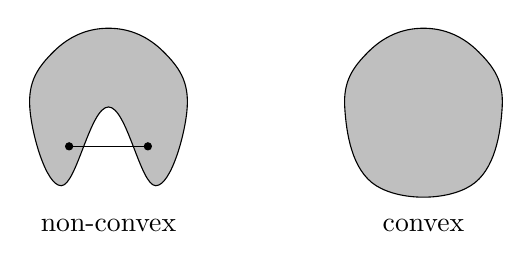
\begin{tikzpicture}
      \begin{scope}[shift={(-2, 0)}]
        \draw [fill=gray!50!white] plot [smooth cycle, tension=0.7] coordinates {(0, 1) (-0.7, 0.7) (-1, 0) (-0.6, -1) (0, 0) (0.6, -1) (1, 0) (0.7, 0.7)};
        \draw (-0.5, -0.5) node [circ] {} -- (0.5, -0.5) node [circ] {};

        \node at (0, -1.5) {non-convex};
      \end{scope}

      \begin{scope}[shift={(2, 0)}]
        \draw [fill=gray!50!white] plot [smooth cycle, tension=0.7] coordinates {(0, 1) (-0.7, 0.7) (-1, 0) (-0.6, -1) (0.6, -1) (1, 0) (0.7, 0.7)};
        \node at (0, -1.5) {convex};
      \end{scope}
    \end{tikzpicture}
  \end{center}
\end{defi}

\begin{defi}[Convex function]
  A function $f: \R^n \to \R$ is \emph{convex} if
  \begin{enumerate}
    \item The domain $D(f)$ is convex
    \item The function $f$ lies below (or on) all its chords, ie.
      \[
        f((1 - t)\mathbf{x} + t\mathbf{y}) \leq (1 - t)f(\mathbf{x}) + tf(\mathbf{y}). \tag{$*$}
      \]
  \end{enumerate}
  A function is \emph{strictly convex} if the inequality is strict, ie.
  \[
    f((1 - t)\mathbf{x} + t\mathbf{y}) < (1 - t)f(\mathbf{x}) + tf(\mathbf{y}).
  \]
  for all $t\in (0, 1)$.
  \begin{center}
    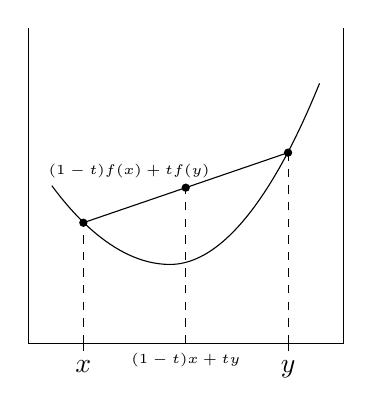
\begin{tikzpicture}
      \draw(-2, 4) -- (-2, 0) -- (2, 0) -- (2, 4);
      \draw (-1.3, 0.1) -- (-1.3, -0.1) node [below] {$x$};
      \draw (1.3, 0.1) -- (1.3, -0.1) node [below] {$y$};
      \draw (-1.7, 2) parabola bend (-.2, 1) (1.7, 3.3);
      \draw [dashed] (-1.3, 0) -- (-1.3, 1.53) node [circ] {};
      \draw [dashed] (1.3, 0) -- (1.3, 2.42) node [circ] {};
      \draw (-1.3, 1.53) -- (1.3, 2.42);
      \draw [dashed] (0, 0) node [below] {\tiny $(1 - t)x + ty$} -- (0, 1.975) node [above] {\tiny$(1 - t)f(x) + t f(y)\quad\quad\quad\quad\quad\quad$} node [circ] {};
    \end{tikzpicture}
  \end{center}

  A function $f$ is (strictly) concave iff $-f$ is (strictly) convex.
\end{defi}

\begin{eg}\leavevmode
  \begin{enumerate}
    \item $f(x) = x^2$ is strictly convex.
    \item $f(x) = |x|$ is convex, but not strictly
    \item $f(x) = \frac{1}{x}$ defined on $x > 0$ is strictly convex.
    \item $f(x) = \frac{1}{x}$ defined on $\R^* = \R \setminus \{0\}$ is \emph{not} convex. Apart from the fact that $\R^*$ is not a convex domain. But even if we defined, like $f(0) = 0$, it is not convex by considering the line joining $(-1, -1)$ and $(1, 1)$ (and in fact $f(x) = \frac{1}{x}$ defined on $x < 0$ is concave).
  \end{enumerate}
\end{eg}
\subsubsection{First-order convexity condition}
Now assume that the function is differentiable. Then we have the first-order condition for convexity. Assume $f$ is (at least) once-differentiable. It is convex if
\[
  h(t) = (1 - t)f(\mathbf{x}) + tf(\mathbf{y}) - f((1 - t)\mathbf{x} + f(\mathbf{y})) \geq 0.
\]
We have $h(0) = 0$. So
\[
  \frac{h(t) - h(0)}{t} \geq 0
\]
for any $t\in (0, 1)$. So
\[
  h'(0) \geq 0.
\]
On the other hand,
\[
  h'(0) = f(\mathbf{y}) - f(\mathbf{x}) - (\mathbf{y} - \mathbf{x})\nabla f (\mathbf{x}).
\]
So convexity implies that
\[
  f(\mathbf{y}) \geq f(\mathbf{x}) + (\mathbf{y} - \mathbf{x})\nabla f(\mathbf{x}) \tag{$\dagger$}
\]
It is also true that $(\dagger)\Rightarrow (*)$, which is an easy exercise. So a convex differentiable function lies above all its tangent planes.

\begin{cor}
  A stationary point of a convex function is a global minimum. There can be more than one global minimum (eg a constant function), but there is at most one if the function is strictly convex.
\end{cor}

\begin{proof}
  Given $\mathbf{x}_0$ such that $\nabla f(\mathbf{x}_0) = \mathbf{0}$, $(\dagger)$ implies that for any $\mathbf{y}$,
  \[
    f(\mathbf{y}) \geq f(\mathbf{x_0}) + (\mathbf{y} - \mathbf{x}_0)\nabla f(\mathbf{x}_0) = f(\mathbf{x}_0).
  \]
\end{proof}

We can rewrite $(\dagger)$ to say
\[
  (\mathbf{y} - \mathbf{x}) \cdot [\nabla f(\mathbf{y}) - \nabla f(\mathbf{x})] \geq f(\mathbf{x}) - f(\mathbf{y}) - (\mathbf{x} - \mathbf{y}) \cdot \nabla f(\mathbf{y}).
\]
But the right is $\geq 0$ by $\dagger$. So we have another first-order condition:
\[
  (\mathbf{y} - \mathbf{x})\cdot [\nabla f(\mathbf{y}) - \nabla f(\mathbf{x})]  \geq 0,
\]
It can be shown that this is equivalent to the other conditions.

This should be interpreted as ``$\nabla f(\mathbf{x})$ is a non-decreasing function''. For example, when $n = 1$, we have $(y - x)(f'(y) - f'(x)) \geq 0$, which implies that $f'(y) > f'(x)$ for $y > x$.

\subsubsection{Second-order convexity condition}
Assume that $f$ is (at least) twice differentiable.

In the last condition we had, let $\mathbf{y} = \mathbf{x} + \mathbf{h}$. Then
\[
  \mathbf{h} \cdot (\nabla f(\mathbf{x} + \mathbf{h}) - \nabla f(\mathbf{x})) \geq 0.
\]
Expand the left in Taylor series. Then the left hand side is
\[
  h_i [h_j \nabla_j \nabla_i f + O(h^2)]
\]
But $\nabla_j \nabla_i f = H_{ij}$. So we have
\[
  h_i H_{ij}h_j + O(h^3) \geq 0
\]
This is true for all $h$ if the Hessian $H$ is positive, ie. the eigenvalues are non-negative. If they are in fact all positive, then we say $H$ is positive definite.

Hence convexity implies that the Hessian matrix is positive for all $\mathbf{x}\in D(f)$. Strict convexity implies that it is positive definite.

The converse is also true - if the Hessian is positive definite, then it is convex.

\begin{eg}
  Let $f(x, y) = \frac{1}{xy}$ for $x, y > 0$. Then the Hessian is
  \[
    H = \frac{1}{xy}
    \begin{pmatrix}
      \frac{2}{x^2} & \frac{1}{xy}\\
      \frac{1}{xy} & \frac{2}{y^2}
    \end{pmatrix}
  \]
  The determinant is
  \[
    \det H = \frac{3}{x^4y^4} > 0
  \]
  and the trace is
  \[
    \tr H = \frac{2}{xy}\left(\frac{1}{x^2} + \frac{1}{y^2}\right) > 0.
  \]
  So $f$ is convex.

  We only relied on $xy$ being positive. Can we relax the domain condition to be $xy > 0$ instead? No! This is because the domain will no longer be convex! 
\end{eg}

\subsection{Legendre transform}
\begin{defi}[Legendre transform]
  Given a function $f: \R^n \to \R$, its \emph{Legendre transform} $f^*$ (the ``conjugate'' function) is defined by
  \[
    f^*(\mathbf{p}) = \sup_{x}(\mathbf{p}\cdot \mathbf{x} - f(\mathbf{x})),
  \]
  The domain of $f^*$ is the set of $\mathbf{p}\in \R^n$ such that the supremum is finite.
\end{defi}
It follows immediately that
\begin{lemma}
  $f^*$ is always convex.
\end{lemma}

\begin{proof}
  \begin{align*}
    f^*((1 - t)\mathbf{p} + t\mathbf{q}) &= \sup_x \big[((1 - t)\mathbf{p}\cdot \mathbf{x} + t\mathbf{q}\cdot \mathbf{x} - f(\mathbf{x})\big].\\
    &= \sup_x \big[(1 - t)(\mathbf{p}\cdot \mathbf{x} - f(\mathbf{x})) + t(\mathbf{q}\cdot \mathbf{x} - f(\mathbf{x}))\big]\\
    &\leq (1 - t)\sup_x [\mathbf{p}\cdot \mathbf{x} - f(\mathbf{x})] + t\sup_x[\mathbf{q}\cdot \mathbf{x}  - f(\mathbf{x})]\\
    &= (1 - t)f^*(\mathbf{p}) + tf^*(\mathbf{q})\\
  \end{align*}
  Note that we cannot immediately conclude that $f$ is convex, since we have to show that the domain is convex. But by the above bounds, $f^*((1 - t)\mathbf{p} + t\mathbf{q})$  is bounded by the sum of two finite terms, which is finite. So $(1 - t)\mathbf{p} + t\mathbf{q}$ is also in the domain of $f$.
\end{proof}

Now suppose that $f(\mathbf{x})$ is differentiable. Then the maximum of the right hand side is found by solving (for $\mathbf{x}$ as a function of $\mathbf{p}$) $\mathbf{p} = \nabla f(\mathbf{x})$

If $f$ is strictly convex, then a solution of this equation (if exists) is unique.

For example, when $n = 1$, $f^*(p) = px - f(x)$, where $x$ satisfies $f'(x) = p$.

\begin{center}
  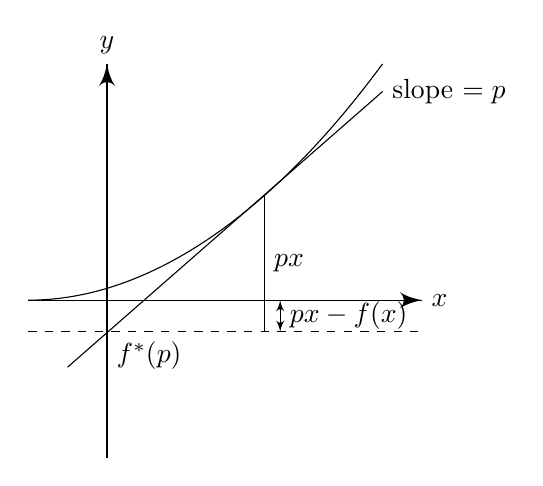
\begin{tikzpicture}
    \draw [->] (-1, 0) -- (4, 0) node [right] {$x$};
    \draw [->] (0, -2) -- (0, 3) node [above] {$y$};
    \draw (-1, 0) parabola (3.5, 3);
    \draw (3.5, 2.65) node [right] {slope $=p$} -- +(-4, -3.5);
    \draw [dashed] (-1, -0.4) -- +(5, 0);
    \node at (0, -0.4) [anchor = north west] {$f^*(p)$};
    \draw (2, -0.4) -- +(0, 1.74) node [pos=0.5, right] {$px$};
    \draw [arrows={latex'-latex'}] (2.2, 0) -- (2.2, -0.4) node [right, pos=0.5] {$px - f(x)$};
  \end{tikzpicture}
\end{center}

\begin{eg}\leavevmode
  \begin{enumerate}
    \item Let $f(x) = \frac{1}{2}ax^2$ for $a > 0$. Then $p = ax$ at the maximum of $px - f(x)$. So
      \[
        f^*(p) = px - f(x) = p\cdot \frac{p}{a} - \frac{1}{2}a\left(\frac{p}{a}\right)^2 = \frac{1}{2a}p^2.
      \]
      So the Legendre transform maps a parabola to a parabola.
    \item $f(v) = -\sqrt{1 - v^2}$ for $|v| < 1$ is a lower semi-circle. We have
      \[
        p = f'(v) = \frac{v}{\sqrt{1 - v^2}}
      \]
      So
      \[
        v = \frac{p}{\sqrt{1 + p^2}}
      \]
      and exists for all $p\in \R$. So
      \[
        f^*(p) = pv - f(v)|_{v = v(p)} = \frac{p^2}{\sqrt{1 + p^2}} + \frac{1}{\sqrt{1 + p^2}} = \sqrt{1 + p^2}.
      \]
      A circle gets mapped to a hyperbola.
    \item Let $f = cx$ for $c > 0$. This is convex but not strictly convex. Then $px - f(x) = (p - c)x$. This has no maximum unless $p = c$. So the domain of $f^*$ is simply $\{c\}$. One point. So $f^*(p) = 0$. So a line goes to a point.
  \end{enumerate}
\end{eg}
\begin{thm}
  If $f$ is convex, differentiable with Legendre transform $f^*$, then $f^{**} = f$. 
\end{thm}

\begin{proof}
  We have $f^*(\mathbf{p}) = (\mathbf{p}\cdot\mathbf{x}(\mathbf{p}) - f(\mathbf{x}(\mathbf{p}))$ where $\mathbf{p} = \nabla f(\mathbf{x}(\mathbf{p}))$.

  Differentiating with respect to $\mathbf{p}$, we have
  \begin{align*}
    \nabla_i f^*(\mathbf{p}) &= x_i + p_j \nabla_i x_j (\mathbf{p}) - \nabla_i x_j(\mathbf{p}) \nabla_j f(\mathbf{x})\\
    &= x_i + p_j \nabla_i x_j(\mathbf{p}) - \nabla_i x_j(\mathbf{p}) p_j\\
    &= x_i.
  \end{align*}
  So
  \[
    \nabla f^*(\mathbf{p}) = \mathbf{x}.
  \]
  Hence
  \begin{align*}
    \nabla f(\mathbf{x}) = \mathbf{p} &\Rightarrow \mathbf{x} = \mathbf{x}(\mathbf{p})\\
    \nabla f^*(\mathbf{p}) = \mathbf{x} &\Rightarrow \mathbf{p} = \mathbf{p}(\mathbf{x}).
  \end{align*}
  Now we take the Legendre transform of $f^*$:
  \begin{align*}
    f^{**}(\mathbf{x}) &= (\mathbf{x} \cdot \mathbf{p} - f^*(\mathbf{p}))|_{\mathbf{p} = \mathbf{p}(\mathbf{x})}\\
    &= \mathbf{x}\cdot \mathbf{p} - (\mathbf{p}\cdot \mathbf{x} - f(\mathbf{x}(\mathbf{p}(\mathbf{x}))))\\
    &= f(\mathbf{x}).
  \end{align*}
\end{proof}
\note if $f = (f^*)^*$, then $f$ is convex since it is a Legendre transform. So the convexity condition is really required for the theorem.

Note that strict convexity is \emph{not} required. For example, in our last example above, $f^*(p) = 0$ for $p = c$. So $f^{**}(x) = (xp - f^*(p))|_{p = c} = cx = f(x)$.

\subsection{Application to thermodynamics}
For a system in thermal equilibrium at temperature $T$ and pressure $P$, the first law of thermodynamics says that
\[
  \d E = T\;\d S - p\;\d V.
\]
Here $T\;\d S = \d Q$ is the heat change, and $-p\;\d V = \d W$ is the work done.

From this, we obtain
\[
  \frac{\partial E}{\partial S} = T,\quad \frac{\partial E}{\partial V} = p
\]
We say that $S$ and $V$ \emph{extensive} variables - they scale with the system; $T$ and $p$ are \emph{intensive} variables.

On the right hand side of the first law, variables come in conjugate pairs, eg. $(T, S)$, $(p, V)$. In other cases, we have like $(\mu, N)$, the chemical potential and number of particles.

To find the equilibrium at fixed $S$, we minimize $E$. But in practice, we fix $T$ and not $S$, ie. we put in contact with a heat reservoir.

In this case, it is the \emph{Helmholtz free energy}
\[
  F(T, V) = E(S, V) - TS = E(S, V) - S\frac{\partial E}{\partial S}.
\]
that is minimized. We see that $F(T, V)$ is the Legendre transform of $-E(S, V)$.

If we get the Legendre transform with respect to $V$, we get the enthalpy instead.

\section{Lagrange multipliers}
Let $f(x, y)$ be the height above ground. The hill tip is at the max of $f$, which satisfies
\[
  0 = \d f = \nabla f\cdot \d \mathbf{\ell}
\]
for all $\d \mathbf{\ell}$. So we need
\[
  \nabla f = 0.
\]
However, suppose we have a particular path $p$ defined by $p(x, y) = 0$. Where is the highest point on the path $p$?

We still need $\nabla f \cdot \d \mathbf{\ell} = 0$, but now $\d \mathbf{\ell}$ is \emph{not} arbitrary, but only for $\d \ell$ that is parallel to the path. Alternatively, $\nabla f$ has to be entirely perpendicular to the path. Since we know that the normal to the path is $\nabla p$, our condition becomes
\[
  \nabla f = \lambda \nabla p
\]
for some lambda $\lambda$. Of course, we still have the constraint $p(x, y) = 0$. So what we have to solve is
\begin{align*}
  \nabla f &= \lambda \nabla p\\
  p &= 0
\end{align*}
for the three variables $x, y, \lambda$.

Alternatively, we can solve for the stationary points of the function $\phi(x, y, \lambda)$ given by
\[
  \phi(x, y, \lambda) = f(x, y) - \lambda p(x, y)
\]
Now we have changed constrained maximization problem to a problem of unconstrained extremization.

\begin{eg}
  Find the radius of the smallest circle centered on origin that intersects $y = x^2 - 1$.

  \begin{enumerate}
    \item  First do it the easy way: for a circle of radius $R$ to work, $x^2 + y^2 = R^2$ and $y = x^2 - 1$ must have a solution. So
      \[
        (x^2)^2 - x^2 + 1 - R^2 = 0
      \]
      and
      \[
        x^2 = \frac{1}{2}\pm \sqrt{R^2 - \frac{3}{4}}
      \]
      So $R_{\min} = \sqrt{3}/2$.

    \item We can also view this as a variational problem. We want to minimize $f(x, y) = x^2 + y^2$ subject to the constraint $p(x, y) = 0$ for $p(x, y) = y - x^2 + 1$.

      We can solve this directly. We can solve the constraint to obtain $y = x^2 - 1$. Then 
      \[
        R^2(x) = f(x, y(x)) = (x^2)^2 - x^2  + 1
      \]
      We look for stationary points of $R^2$:
      \[
        (R^2(x))' = 0 \Rightarrow  x\left(x^2 - \frac{1}{2}\right)= 0
      \]
      So $x = 0$ and $R = 1$; or $x = \pm \frac{1}{\sqrt{2}}$ and $R = \frac{\sqrt{3}}{2}$. Since $\frac{\sqrt{3}}{2}$ is smaller, this is our minimum.

    \item Finally, we can use Lagrange multipliers. We find stationary points of the function 
      \[
        \phi(x, y, \lambda) = f(x, y) - \lambda p(x, y) = x^2 + y^2 - \lambda (y - x^2 + 1)
      \]
      The partial derivatives give
      \begin{align*}
        \frac{\partial \phi}{\partial x} = 0 &\Rightarrow 2x(1 + \lambda) = 0\\
        \frac{\partial \phi}{\partial y} = 0 &\Rightarrow 2y - \lambda = 0\\
        \frac{\partial \phi}{\partial \lambda} = 0 &\Rightarrow y - x^2 + 1 = 0
      \end{align*}
      The first equation gives us two choices: If $x = 0$, then $y = -1$. So $\lambda = -1$. Then $R = 1$.

      If $\lambda = -1$, we have $y = -\frac{1}{2}$ and $x = \pm \frac{1}{\sqrt{2}}$. So $R = \frac{\sqrt{3}}{2} < 1$ is the minimum.
  \end{enumerate}
\end{eg}
This can be generalized to problems with functions $\R^n \to \R$ using the same logic.

\begin{eg}
  For $x\in \R^n$, find the minimum of the quadratic form
  \[
    f(x) = x_i A_{ij}x_j
  \]
  on the surface $|\mathbf{x}|^2 = 1$.

  \begin{enumerate}
  \item The constraint imposes a normalization condition $\mathbf{x}$. But if we scale up $\mathbf{x}$, $f(\mathbf{x})$ scales accordingly. So if we define
    \[
      \Lambda(\mathbf{x}) = \frac{f(\mathbf{x})}{g(\mathbf{x})},\quad g(\mathbf{x}) = |\mathbf{x}|^2
    \]
    The problem is equivalent to minimization of $\Lambda (\mathbf{x})$ without constraint. Then
    \[
      \nabla_i \Lambda(\mathbf{x}) = \frac{2}{g}\left[A_{ij} x_j - \frac{f}{g} x_i\right]
    \]
    So we need
    \[
      A\mathbf{x} = \Lambda \mathbf{x}
    \]
    So the extremal values of $\Lambda (\mathbf{x})$ are the eigenvalues of $A$. If $A$ is positive, then $\Lambda_{\min}$ is the lowest eigenvalue.

  \item We can also do it with Lagrange multipliers. We want to find stationary values of 
    \[
      \phi(\mathbf{x}, \lambda) = f(\mathbf{x}) - \lambda(|\mathbf{x}|^2 - 1).
    \]
    So
    \[
      0 = \nabla \phi \Rightarrow  A_{ij} x_j = \lambda x_i
    \]
    Differentiating with respect to $\lambda$ gives
    \[
      \frac{\partial \phi}{\partial \lambda} = 0 \Rightarrow  |\mathbf{x}|^2 = 1.
    \]
    So we get the same set of equations.
  \end{enumerate}
\end{eg}

\begin{eg}
  What probability distribution $\{p_1, \cdots, p_n\}$ satisfying $\sum_i p_i = 1$ maximizes the information entropy
  \[
    S = - \sum_{i = 1}^n p_i \log p_i
  \]
  We look for stationary points of
  \[
    \phi(\mathbf{p}, \lambda) = -\sum_{i = 1}^n p_i \ln p_i - \lambda\sum_{i = 1}^n p_i + \lambda.
  \]
  We have
  \[
    \frac{\partial \phi}{\partial p_i}= - \ln p_i - (1 + \lambda) = 0
  \]
  So
  \[
    p_i = e^{-(1 + \lambda)}
  \]
  It's the same for all $i$! So we must have $p_i = \frac{1}{n}$.
\end{eg}
\section{Functionals and Euler-Lagrange equation}
\begin{defi}[Functional]
  A functional is a function that takes in another real-valued function as an argument. We usually write them as
  \[
    F[ x] \in \R
  \]
  where $x = x(s): \R \to \R$. We say that $F[ x]$ is a functional of the function $x(s)$.
\end{defi}

Note that $F[x]$ depends on the function $x(s)$, but not on its independent variable $s$.

Of course, we can also have functionals of many functions, eg. $F[x, y]\in \R$ for $x, y: \R \to \R$. We can also have functionals of a function of many variables.

There is a particular class of functionals that we care about. We start with $F[y]$ for a single function $y(x)$ defined for $\alpha \leq x \leq \beta$.

Most of the time, our functional is of the form
\[
  F[y]  = \int_\alpha ^\beta f(y, y', x)\;\d x
\]
for some function $f$. Note that the integrand can also depend on $y''$, $y'''$ etc, but it usually doesn't.

$f$ has an \emph{implicit} dependence on $x$ through $y$, but also (possibly) an \emph{explicit} dependence on $x$.

Now we investigate how $F[y]$ changes if we change $y: y(x) \mapsto y(x) + \delta y(x)$.

The change $\delta F[y]$ of $F[y]$ is
\begin{align*}
  \delta F[y] &= F[y + \delta y] - F[y]\\
  &= \int_\alpha ^\beta \big(f(y + \delta y, y' + \delta y', x) - f(y, y', x)\big)\;\d x\\
  \intertext{Taylor expand to obtain}
  &= \int_\alpha^\beta  \left(\delta y\frac{\partial f}{\partial y} + \delta y' \frac{\partial f}{\partial y'}\right)\;\d x + o(\delta^2)\\
  \intertext{Integrate the second term by parts to obtain}
  \delta F[y] &= \int_\alpha^\beta\delta y\left[\frac{\partial f}{\partial y} - \frac{\d}{\d x}\left(\frac{\partial f}{\partial y'}\right)\right]\;\d x + \left[ \delta y\frac{\partial f}{\partial y'}\right]_\alpha^\beta.
\end{align*}
This huge scary expression can be simplified if the second term (the \emph{boundary term}) vanishes, and fortunately this is true for most interesting boundary conditions, such as
\begin{itemize}
  \item Fix $y$ at $x = \alpha, \beta$, so $\delta y(\alpha) = \delta y(\beta) = 0$.
  \item Usually $y' = 0 \Rightarrow \frac{\partial f}{\partial y'} = 0$. So we can set our boundary condition as $y'(\alpha) = y'(\beta) = 0$.
  \item We can mix both of them, eg. set $y(\alpha) =$ constant and $y'(\beta) = 0$.
\end{itemize}
Regardless of what we do, we choose boundary conditions such that the boundary term is 0. Then
\[
  \delta F[y] = \int_\alpha ^\beta \left(\delta y \frac{\delta F[y]}{\delta y(x)}\right)\;\d x
\]
where
\begin{defi}[Functional derivative]
  \[
    \frac{\delta F[y]}{\delta y} = \frac{\partial f}{\partial y} - \frac{\d }{\d x}\frac{\partial f}{\partial y'}
  \]
  is the \emph{functional derivative} of $F[y]$.
\end{defi}

If we want to find a minimum or maximum of $F$, then we need $\frac{\delta F[y}{\delta y} = 0$. So
\begin{defi}[Euler-Lagrange equation]
  The \emph{Euler-Lagrange} equation is
  \[
    \frac{\partial f}{\partial y} - \frac{\d}{\d x}\left(\frac{\partial f}{\partial  y'}\right) = 0
  \]
  for $\alpha \leq x \leq \beta$.
\end{defi}
There is an obvious generalization to functionals $F[\mathbf{y}]$  for $\mathbf{y}(x) \in \R^n$:
\[
  \frac{\partial f}{\partial y_i} - \frac{\d }{\d x}\left(\frac{\partial f}{\partial y_i'}\right) = 0
\]
for all $i$ and $\alpha \leq x \leq \beta$.
\begin{eg}[Geodesics of a plane]
  What is the curve $C$ of minimal length between two points $A, B$ in the Euclidean plane? The length is
  \[
    L = \int_C \;\d \ell
  \]
  where $\;\d \ell = \sqrt{\d x^2 + \d y^2}$.

  There are two ways we can do this:
  \begin{enumerate}
    \item We restrict to curves for which $x$ (or $y$) is a good parameter, ie. $y$ can be made a function of $x$. Then
      \[
        \d \ell = \sqrt{1 + (y')^2}\;\d x.
      \]
      Then
      \[
        L[y] = \int_\alpha^\beta \sqrt{1 + (y')^2}\;\d x.
      \]
      We see that
      \[
        \frac{\partial f}{\partial y} = 0
      \]
      and we have fixed end points. So the Euler-Lagrange equation says that
      \[
        \frac{\d}{\d x} \left(\frac{\partial f}{\partial y'}\right) = 0
      \]
      So
      \[
        \frac{y'}{\sqrt{1 + (y')^2}} = \text{constant}
      \]
      This is called the first integral of the Euler-Lagrange equation. So $y'$ is a constant. So $y = ax + b$, ie. a straight line.
    \item Get around the restriction to ``good'' curves by choosing an arbitrary parameterization $\mathbf{r} = (x(s), y(s))$ for $s\in [0, 1]$ such that $\mathbf{r}(0) = A$, $\mathbf{r}(1) = B$. So
      \[
        \d \ell = \sqrt{\dot x^2 + \dot y^2}\;\d s.
      \]
      Now
      \[
        L[x, y] = \int_0^1 \sqrt{\dot x^2 + \dot y^2} \;\d s.
      \]
      We have, again
      \[
        \frac{\partial f}{\partial x} = \frac{\partial f}{\partial y} = 0.
      \]
      So we are left to solve
      \[
        \frac{\d }{\d s}\left(\frac{\partial f}{\partial \dot x}\right) = \frac{\d }{\d s}\left(\frac{\partial f}{\partial \dot y}\right)  = 0.
      \]
      So
      \[
        \frac{\dot x}{\sqrt{\dot x^2 + \dot y^2}} = c
      \]
      and
      \[
        \frac{\dot y}{\sqrt{\dot x^2 + \dot y^2}} = s
      \]
      where $c$ and $s$ are constants. But these constants are not independent, since we have $c^2 + s^2 = 1$.So let $c = \cos \theta$, $s = \sin \theta$. Then the two conditions are both equivalent to
       
      \[
        (\dot x \sin \theta)^2 = (\dot y\sin \theta)^2.
      \]
      Then
      \[
        \dot x \sin \theta = \pm\dot y \cos \theta.
      \]
      We can choose $\theta$ such that we have a positive sign. So
      \[
        y\cos \theta = x\sin \theta + A
      \]
      for a constant $A$. So this is a straight line with slope $\tan \theta$.
  \end{enumerate}
\end{eg}
\subsection{First integrals and Fermat's principle}
When $f$ does not depend on $y$, ie.
\[
  F[y] = \int_{x_A}^{x_B} f(y', x)\;\d x,
\]
then $\frac{\partial f}{\partial y} = 0$. Then the Euler-Lagrange equation says
\[
  \frac{\partial f}{\partial y'} = \text{const}
\]
We call this the first integral.

We also get first integrals when $\frac{\partial f}{\partial x} = 0$, ie. when $f$ has no \emph{explicit} dependence on $x$.

By the chain rule,
\[
  \frac{\d f}{\d x} = \frac{\partial f}{\partial x} + y' \frac{\partial f}{\partial y} + y'' \frac{\partial f}{\partial y'}.
\]
Then Euler-Lagrange says that
\[
  \frac{\partial f}{\partial y} = \frac{\d}{\d x} \left(\frac{\partial f}{\partial y'}\right).
\]
So our equation becomes
\begin{align*}
  \frac{\d f}{\d x} &= \frac{\partial f}{\partial x} + y' \frac{\d}{\d x}\left(\frac{\partial f}{\partial y'}\right) + y''\frac{\partial f}{\partial y'}\\
  &= \frac{\partial f}{\partial x} + \frac{\d}{\d x}\left(y'\frac{\partial f}{\partial y'}\right).
\end{align*}
Then
\[
  \frac{\d}{\d x}\left(f - y'\frac{\partial f}{\partial y'}\right) = \frac{\partial f}{\partial x}.
\]
If $\frac{\partial f}{\partial x} = 0$, then we have the first integral
\[
  f - y'\frac{\partial f}{\partial y} = \text{const}
\]
This is useful for many important variational problems.

\begin{eg}
  Consider the path of a light ray in vertical $x-z$ plane inside a medium with refractive index $n(z) = \sqrt{a - bz}$ for positive constants $a, b$. The phase velocity of light is $v = \frac{c}{n}$.

  According the Fermat's principle, the path minimizes
  \[
    T = \int_A^B \frac{\d \ell}{v}.
  \]
  This is equivalent to minimizing
  \[
    cT = P = \int_A^B n\;\d \ell,
  \]
  the optical path length. Write 
  \[
    \;\d \ell = \sqrt{\d x^2 + \d z^2} = \sqrt{1 + z'(x)^2}\;\d x,
  \]
  where the path is specified by the function $z(x)$.

  Then
  \[
    P[z] = \int_{x_A}^{x_B}n(z)\sqrt{1 + (z')^2}\;\d x.
  \]
  Since this does not depend on $x$, the Euler-Lagrange equation implies that
  \[
    k = f - z'\frac{\partial f}{z'} = \frac{n(z)}{\sqrt{1 + (z')^2}}.
  \]
  for an integration constant $k$. Squaring and putting in the value of $n$ gives
  \[
    (z')^2 = \frac{b}{k^2}(z_0 - z),
  \]
  where $z_0 = (a - k^2)/b$. So
  \[
    \frac{\d z}{\sqrt{z_0 - z}} = \pm\frac{\sqrt{b}}{k}\;\d x.
  \]
  So
  \[ \sqrt{z - z_0} = \pm \frac{b}{2k^2}(x - x_0),
  \]
  where $x_0$ is our second integration constant. Square it to obtain
  \[
    z = z_0 - \frac{b}{4k^2}(x - x_0)^2,
  \]
  which is a parabola!
\end{eg}

\begin{eg}[Principle of least action]
  This is turning mechanics into a variational problem.

  At first, Manpotuis proposed that the action should be defined as mass $\times$ velocity $\times$ distance.

  Euler made it more precise. For a particle with constant energy,
  \[
    E = \frac{1}{2} mv^2 + U(\mathbf{x}),
  \]
  where $v = |\dot{\mathbf{x}}|$. So we have
  \[
    mv = \sqrt{2m(E - U(\mathbf{x}))}.
  \]
  Hence we can define the action to be
  \[
    A = \int_A^B \sqrt{2m(E - U(x))}\;\d \ell,
  \]
  where $\d\ell = \sqrt{\d x^2 + \d z^2}$. We minimize this to find the trajectory.

  For a particle near the surface of the Earth, under the influence of gravity, $U = mgz$. So we have
  \[
    A[z] = \int_A^B \sqrt{2mE - 2m^2gz}\sqrt{1 + (z')^2}\;\d x,
  \]
  which is of exactly the same form as the optics problem we just solved. So the result is again a parabola, as expected.
\end{eg}
\note this is the 18th century version of the action. In the 19th century, Hamilton gave a better definition that was much easier to work with.

\begin{eg}[Branchistochrone]
  We have a bead sliding along a frictionless wire. We suppose it starts from rest at the origin $A$. What shape of wire minimizes the time for the bead to travel from $A$ to $B$?

  \begin{center}
    \begin{tikzpicture}
      \draw [->] (-0.5, 0) -- (4, 0) node [right] {$x$};
      \draw [->] (0, 0.5) -- (0, -3) node [below] {$y$};

      \draw [red] (0.86, -1) circle [radius=0.1];

      \node [circ] {};
      \node [anchor = south east] {$A$};

      \node at (3, -1) [circ] {};
      \node at (3, -1) [right] {$B$};
      \draw (0, 0) parabola bend (2, -1.5) (3, -1);
    \end{tikzpicture}
  \end{center}

  The conservation of energy implies that
  \[
    \frac{1}{2}mv^2 = mgy.
  \]
  So
  \[
    v = \sqrt{2gy}
  \]
  We want to minimize
  \[
    T = \int \frac{\d \ell}{v}.
  \]
  So
  \[
    T = \frac{1}{\sqrt{2g}}\int \frac{\sqrt{\d x^2 + \d y^2}}{\sqrt{y}} = \sqrt{\frac{1 + (y')^2}{y}}\;\d x
  \]
  Since there is no explicit dependence on $x$, we have the first integral
  \[
    f - y'\frac{\partial f}{\partial y} = \frac{1}{\sqrt{y(1 + (y')^2)}} = \text{constant}
  \]
  So the solution is
  \[
    y(1 + (y')^2) = c
  \]
  for some positive constant $c$.

  The solution of this ODE is, in parametric form
  \begin{align*}
    x &= c(\theta - \sin \theta)\\
    y &= c(1 - \cos \theta).
  \end{align*}
  Note that this has $x = y = 0$ at $\theta = 0$. This describes a cycloid.
\end{eg}

\section{Constrained variation of functionals}
The problem is to find stationary values of $F[y]$ subject to the constraint $P[y] = c$ for some constant $c$.

We can again use Lagrange multipliers. The problem is equivalent to finding stationary values (without constraints) of
\[
  \Phi_\lambda [y] = F[y] - \lambda(P[y] - c).
\]
with respect to the function $y(x)$ and the variable $\lambda$.

\begin{eg}[Isoperimetric problem]
  What is the simple closed curved in the plane of fixed length $L$ that maximizes the enclosed area? (simple means connected and not self-intersecting)

  We assume that the curve encloses a region that is convex (if it is not convex, we can ``push out'' the curve to increase the area without changing the length).

  We can split the curve into two parts:
  \begin{center}
    \begin{tikzpicture}
      \draw [red] plot [smooth, tension=1.2] coordinates {(1, 1.5) (1.6, 2.3) (2.6, 1.8)  (3.5, 2) (4, 1.5)};
      \node [red, anchor = south east] at (1.2, 1.75) {$y_2$};
      \draw [blue] plot [smooth, tension=1.2] coordinates {(1, 1.4) (1.4, 0.8) (2.6, 1) (3.6, 0.9) (4, 1.5)};
      \node [blue, anchor = north west] at (3, 0.8) {$y_1$};

      \draw [dashed] (1, 1.5) -- (1, 0) node [below] {$\alpha$};
      \draw [dashed] (4, 1.5) -- (4, 0) node [below] {$\beta$};

      \draw [->] (0, 0) -- (5, 0) node [right] {$x$};
      \draw [->] (0, 0) -- (0, 3) node [above] {$y$};
    \end{tikzpicture}
  \end{center}

  We have $\d A = [y_2(x) - y_1(x)]\;\d x$. So
  \[
    A = \int_\alpha^\beta [y_2(x) - y_1(x)]\;\d x.
  \]
  So
  \[
    A[y] = \oint y(x)\;\d x.
  \]
  and the length is
  \[
    L[y] = \oint d\ell = \oint \sqrt{1 + (y')^2}\;\d x.
  \]
  So we look for stationary points of
  \[
    \Phi_\lambda [y] = \oint [y(x) - \lambda\sqrt{1 + (y')^2}]\;\d x + \lambda L.
  \]
  Note that there is no boundary term because there is no boundary. Also, $\frac{\partial f}{\partial x} = 0$. So we get the first integral
  \[
    f - y'\frac{\partial f}{\partial y'} = \text{const} = y_0.
  \]
  So
  \[
    y_0 = y - \lambda\sqrt{1 + (y')^2} - \frac{\lambda (y')^2}{\sqrt{1 + (y')^2}} = y - \frac{\lambda}{\sqrt{1 + (y')^2}}.
  \]
  So
  \begin{align*}
    (y - y_0)^2 &= \frac{\lambda^2}{1 + (y')^2}\\
    (y')^2 &= \frac{\lambda^2}{(y - y_0)^2} - 1\\
    \frac{(y - y_0)y'}{\sqrt{\lambda^2 - (y - y_0)^2}} &= \pm 1.\\
    \d\left[\sqrt{\lambda^2 - (y - y_0)^2}\pm x\right] &= 0.\\
  \end{align*}
  So we have
  \[
    \lambda^2 - (y - y_0)^2 = (x - x_0)^2.
  \]
  So
  \[
    (x - x_0)^2 + (y - y_0)^2 = \lambda^2.
  \]
  So this is a circle of radius $\lambda$. Since the perimeter of this circle will be $2\pi \lambda$, we must have $\lambda = L/(2\pi)$. So the maximum area is $\pm \lambda^2 = L^2/(4\pi)$.
\end{eg}

\begin{eg}[Sturm-Liouville problem]
  Let 
  \[
    F[y] = \int_\alpha^\beta (\rho(x)(y')^2 + \sigma(x)y^2)\;\d x
  \]
  and
  \[
    G[y] = \int_\alpha^\beta w(x)y^2\;\d x.
  \]
  for $\rho, w> 0$ when $\alpha < x < \beta$.

  Find the stationary values of $F[y]$ subject to the constraint $G = 1$, given that $y(x)$ is fixed at $x = \alpha, \beta$.

  From the Euler-Lagrange equation, we have
  \begin{align*}
    \frac{\delta F[y]}{\delta y} &= 2\big(-(\rho y')' + \sigma y\big)\\
    \frac{\delta G[y]}{\delta y} &= 2 (wy).
  \end{align*}
  So The Euler-Lagrange equation of $\Phi_\lambda [y] = F[y] - \lambda(G[y] - 1)$ is
  \[
    -(\rho y')' + \sigma y - \lambda wy = 0.
  \]
  or
  \[
    \mathcal{L}y = \lambda wy.
  \]
  where
  \[
    L = -\frac{\d}{\d x}\left(\rho\frac{\d}{\d x}\right) + \sigma
  \]
  is the \emph{Sturm-Liouville operator}. So this is an Sturm-Liouville eigenvalue problem. $w$ is called the \emph{weight function}.

  Notice that $\lambda y = \lambda wy$ is \emph{linear} in $y$, so if $y$ is a solution, so is $Ay$. But if $G[y ] = 1$, then $G[Ay] = A^2$. So the constraint just fixes the normalization of $y$. But this drops out of the ratio
  \[
    \Lambda [y] = \frac{F[y]}{G[y]}
  \]
  So we can find the stationary points of this instead. Suppose now that $\sigma(x) > 0$. Then $F[y] \geq 0$. So
 \[
    \Lambda = \frac{F}{G} \geq 0.
  \]
  So $\Lambda[y]$ has a minimum. To find the stationary points of $\lambda$, we have
  \[
    \delta\Lambda = \frac{1}{G}\delta F - \frac{F}{G^2} \delta G = \frac{1}{G}(\delta F - \Lambda \delta G).
  \]
  So
  \[
    \Delta \Lambda = 0 \Leftrightarrow \frac{\delta F}{\delta y} = \Lambda \frac{\delta G}{\delta y} \Rightarrow \mathcal{L} y = \Lambda y.
  \]
  So the minimum value of $\Lambda[y]$ is the lowest Sturm-Liouville eigenvalue.
\end{eg}

\begin{eg}[Functional constraint - geodesics]
  Let $\E^n$ be $\R^n$ with Euclidean metric $\d \ell^2 = \sum \d x_i^2$.

  Let $S$ be a hypersurface in $\E^n$ be defined by $g(\mathbf{x}) = 0$. For example, if $g(\mathbf{x}) = |\mathbf{x}|^2 - 1$, we have a unit sphere.

  We want to find the path of shortest distance between two points. We can either solve $g(x) = 0$, eg. parametrically by, say $x = \cos \theta \cos \phi$, $y = \cos \theta \sin \phi$, $z = \sin \theta$ for $S^2$ in $\E^3$. We then substitute this into $\d \ell$ to get a distance formula on $S$, eg.
  \[
    D[\theta, \phi] = \int_A^B \sqrt{\d \theta^2 + \sin^2 \theta \d \phi^2}
  \]
  Then we minimize $D$ to obtain a geodesic.

  Alternatively, we impose $g(x(t)) = 0$ with Lagrange multiplier $\lambda(t)$. So the problem is equivalent to finding stationary values of
  \[
    \Phi[x, \lambda] = \int_0^1 \big(|\dot{\mathbf{x}}| - \lambda(t) g(x(t))\big)\;\d t
  \]
\end{eg}
\section{Hamilton's principle}
Lagrange in 1788 pointed out that the motion of any dynamical system is a path in multidimensional \emph{configuration space}, where possible every configuration is denoted by some coordinates $\xi$. The path is then $\xi(t)$.

The configuration space is formed by taking all independent parameters describing the particles and putting them into one huge variable. For example, if we have $N$ particles, the configuration space has dimension $3N$, since each particle needs $x, y, z$ coordinates to denote the position, and there are $N$ of these.

If we have molecules, we might have to take into account the rotation, chirality etc of the molecules as well.

Lagrange showed that $\xi(t)$ obeys certain ODEs, and showed that the ODEs are determined by the kinetic energy and the potential energy.

In the 1830s, Hamilton showed that the solutions of these ODEs are extremal points of a new ``action'',
\[
  I[\xi] = \int L\;\d t
\]
where
\[
  L = T - V
\]
is the \emph{Lagrangian}, with $T$ the kinetic energy and $V$ the potential energy.

Hamilton's principle is that the path $\xi(t)$ makes $I$ stationary.

Note that $I$ has dimensions $ML^2T^{-1}$, which is the same as the 18-th century action (and Plank's constant).

\begin{eg}
  Suppose we have 1 particle in Euclidean 3-space. The configuration space is simply the coordinates of the particle in space. We can choose Cartesian coordinates $\mathbf{x}$. Then
  \[
    T = \frac{1}{2}m|\dot{\mathbf{x}}|,\quad V = V(\mathbf{x}, t)
  \]
  and
  \[
    I[\mathbf{x}] = \int_{t_A}^{t_B}\left(\frac{1}{2}m|\dot{\mathbf{x}}|^2 - V(\mathbf{x}, t)\right)\;\d t.
  \]
  Then the Lagrangian is
  \[
    L(\mathbf{x}, \dot{\mathbf{x}}, t) = \frac{1}{2}m|\dot{\mathbf{x}}|^2 - V(\mathbf{x}, t)
  \]
  We apply the Euler-Lagrange equations to obtain
  \[
    0 = \frac{\d}{\d t}\left(\frac{\partial L}{\partial \dot{\mathbf{x}}}\right) - \frac{\partial L}{\partial \mathbf{x}} = m\ddot{\mathbf{x}} + \nabla V.
  \]
  So
  \[
    m\ddot{\mathbf{x}} = -\nabla V
  \]
  This is Newton's law $\mathbf{F} = m\mathbf{a}$ with $\mathbf{F} = -\nabla V$.
\end{eg}
Note that this applies even when $V$ is time-dependent. However, if $\frac{\partial V}{\partial T} = 0$, then $\frac{\partial L}{\partial t} = 0$. Then we can obtain a first integral.

As before, the chain rule gives
\begin{align*}
  \frac{\d L}{\d t} &= \frac{\partial L}{\partial t} + \dot{\mathbf{x}}\cdot \frac{\partial L}{\partial \mathbf{x}} + \ddot{\mathbf{x}} \cdot \frac{\partial}{\partial \dot{\mathbf{x}}}\\
  &= \frac{\partial L}{\partial t} + \dot{\mathbf{x}}\cdot \underbrace{\left(\frac{\partial L}{\partial \mathbf{x}} - \frac{\d}{\d t}\left(\frac{\partial L}{\partial \dot{\mathbf{x}}}\right)\right)}_{\displaystyle\frac{\delta I}{\delta x} = 0} +
  \underbrace{\dot{\mathbf{x}} \frac{\d}{\d t}\left(\frac{\partial L}{\partial \dot{\mathbf{X}}}\right) + \ddot{\mathbf{x}}\cdot \frac{\partial L}{\partial \dot{\mathbf{x}}}}_{\displaystyle\frac{\d}{\d t}\left(\dot{\mathbf{x}}\cdot \frac{\partial L}{\partial \dot{\mathbf{x}}}\right)}
\end{align*}
So we have
\[
  \frac{\d}{\d t}\left(L - \dot{\mathbf{x}}\cdot \frac{\partial L}{\partial t}\right) = \frac{\partial L}{\partial t}.
\]
If $\frac{\partial L}{\partial t} = 0$, then
\[
  \dot{\mathbf{x}}\cdot \frac{\partial L}{\partial \dot {\mathbf{x}}} - L = E
\]
For some constant $E$. For example, for one particle,
\[
  E = m|\dot{\mathbf{x}}|^2 - \frac{1}{2}m|\dot{\mathbf{x}}|^2 + V = T + V = \text{total energy}.
\]

\begin{eg}
  Consider a central force field $\mathbf{F} = -\nabla V$, where $V = V(r)$ is independent of time. We use spherical polar coordinates $r, \theta, \phi$, where
  \begin{align*}
    x &= r\sin \theta \cos \phi\\
    y &= r\sin \theta \sin \phi\\
    z &= r\cos \theta.
  \end{align*}
  So
  \[
    T = \frac{1}{2}m|\dot{\mathbf{x}}|^2 = \frac{1}{2}m\left(\dot{r}^2 + r^2(\dot{\theta}^2 + \sin^2 \theta \dot{\phi}^2)\right)
  \]
  So
  \[
    L = \frac{1}{2}\dot{r}^2 + \frac{1}{2}mr^2\big(\dot{\theta}^2 + \sin^2\theta\dot{\phi}^2\big) - V(r).
  \]
  We'll use the fact that motion is planar (a consequence of angular momentum conservation). So wlog $\theta = \frac{\pi}{2}$. Then
  \[
    L = \frac{1}{2}m\dot{r}^2 + \frac{1}{2}mr^2 \dot{\phi}^2 - V(r).
  \]
  Then the Euler Lagrange equations give
  \begin{align*}
    m\ddot{r} - mr\dot{\phi}^2 + V'(r) &= 0\\
    \frac{\d}{\d t}\left(mr^2 \dot{\phi}^2\right) &= 0.
  \end{align*}
  From the second equation, we see that $r^2 \dot\phi = h$ is a constant (angular momentum per unit mass). Then $\dot{\phi} = h/r^2$. So
  \[
    m\ddot{r} - \frac{mh^2}{r^3} + V'(r) = 0.
  \]
  If we let
  \[
    V_{\mathrm{eff}} = V(r) + \frac{mh^2}{2r^2}
  \]
  be the \emph{effective potential}, then we have
  \[
    m\ddot{r} = -V_{\mathrm{eff}}'(r).
  \]
  For example, in a gravitational field, $V(r) = -\frac{GM}{r}$. Then
  \[
    V_{\mathrm{eff}} = m\left(-\frac{GM}{r} + \frac{h^2}{2r^2}\right).
  \]
\end{eg}

\subsection{The Hamiltonian}
The kinetic energy is usually a convex function of $\dot{\mathbf{x}}$. Take the Legendre transformation of $L(\mathbf{x}, \dot{\mathbf{x}}) = T - V$ with respect to $\dot{\mathbf{x}}$. This is called the Hamiltonian.
\[
  H(\mathbf{x}, \mathbf{p}) = \mathbf{p}\cdot \dot{\mathbf{x}} - L(\mathbf{x}, \dot{\mathbf{x}}),
\]
where $\dot{\mathbf{x}}$ satisfies $\mathbf{p} = \frac{\partial L}{\partial \dot{\mathbf{x}}}$. $\mathbf{p}$ is called the \emph{momentum variable}. For example, for the particle, we have
\[
  L = \frac{1}{2}m|\dot{\mathbf{x}}|^2 - V(|\mathbf{x}|, t).
\]
Then
\[
  \mathbf{p} = \frac{\partial L}{\partial \dot{\mathbf{x}}} = m\dot{\mathbf{x}}.
\]
So
\[
  \dot{\mathbf{x}} = \frac{\mathbf{p}}{m}.
\]
So
\begin{align*}
  H(\mathbf{x}, \mathbf{p}) &= \mathbf{p}\cdot \frac{\mathbf{p}}{m} - \frac{1}{2}m\left(\frac{\mathbf{p}}{m}\right)^2 + V(\mathbf{x}, t)\\
  &= \frac{1}{2m}|\mathbf{p}|^2 + V.
\end{align*}
So $H$ is the total energy, but expressed in terms of $\mathbf{x}, \mathbf{p}$, not $\mathbf{x}, \dot{\mathbf{x}}$.

The corollary is that the Lagrangian is the Legendre transform of the Hamiltonian with respect to $\mathbf{p}$. So
\[
  L = \mathbf{p}\cdot \mathbf{x} - H(\mathbf{x}, \mathbf{p})
\]
with
\[
  \dot{\mathbf{x}} = \frac{\partial H}{\partial \mathbf{p}}
\]
So the equivalent action is
\[
  I[\mathbf{x}, \mathbf{p}] = \int (\mathbf{p}\cdot \dot{\mathbf{x}} - H(\mathbf{x}, \mathbf{p}))\;\d t.
\]
This is the phase-space form of the action. The Euler Lagrange equations for these are
\[
  \dot{\mathbf{x}} = \frac{\partial H}{\partial \mathbf{p}}, \quad \dot{\mathbf{p}} = -\frac{\partial H}{\partial \mathbf{x}}
\]
The area element in phase space $\d \mathbf{x}\; \d \mathbf{p}$  has dimensions of action, $ML^2T^{-1}$.

\section{Symmetries and Noether's theorem}
\note In the lectures, the variables used for the functional are $y, y', x$. However, my brain cannot function well when I'm supposed to think of $x$ as the time variable. Hence I use $x, \dot{x}, t$ instead.

Given
\[
  F[x]= \int_\alpha^\beta f(x, \dot{x}, t)\;\d t,
\]
suppose we change variables by the transformation $t \mapsto t^*(t)$ and $x\mapsto x^*(t^*)$. Then we have a new independent variable and a new function. This gives
\[
  F[x] \mapsto F^* [x^*] = \int_{\alpha^*}^{\beta^*} f(x^*, \dot{x}^*, t^*)\;\d t^*
\]
with $\alpha^* = t^*(\alpha)$ and $\beta^* = t^*(\beta)$.

There are some transformations that are particularly interesting:
\begin{defi}[Symmetry]
  If $F^*[x^*] = F[x]$ for all $x$, $\alpha$ and $\beta$, then the transformation $*$ is a \emph{symmetry}.
\end{defi}

This transformation could be a translation of time, space, or a rotation. The exact symmetries $F$ has depends on the form of $f$. For example, if $f$ only depends on the magnitudes of $x$, $\dot{x}$ and $t$, then rotation of space will be a symmetry.

\begin{eg}\leavevmode
  \begin{enumerate}
    \item Consider the transformation $t \mapsto t$ and $x \mapsto x + \varepsilon$ for some small $\varepsilon$. Then
      \[
        F^*[x^*] = \int_\alpha^\beta f(x + \varepsilon, \dot{x}, t)\;\d x = \int_\alpha^\beta \left(f(x, \dot{x}, t) + \varepsilon \frac{\partial f}{\partial x}\right)\;\d x
      \]
      by the chain rule. Hence this transformation is a symmetry if $\frac{\partial f}{\partial x} = 0$.

      However, we also know that if $\frac{\partial f}{\partial x} = 0$, then we have the first integral
      \[
        \frac{\d}{\d t}\left(\frac{\partial f}{\partial \dot{x}}\right) = 0.
      \]
      So $\frac{\partial f}{\partial \dot{x}}$ is a constant of motion.
    \item Consider the transformation $x \mapsto x - \varepsilon$. For the sake of sanity, we will transform $x\mapsto x^*$ such that $x^*(t^*) = x(t)$. Then
      \[
        F^*[x^*] = \int_\alpha^\beta f(x, \dot{x}, t - \varepsilon)\;\d t = \int_\alpha^\beta \left(f(x, \dot{x}, t) - \varepsilon \frac{\partial f}{\partial t}\right)\;\d t.
      \]
      Hence this is a symmetry if $\frac{\partial f}{\partial t} = 0$.

      We also know that if $\frac{\partial f}{\partial t} = 0$ is true, then we obtain a different first integral
      \[
        \frac{\d}{\d t}\left(f - \dot{x}\frac{\partial f}{\partial \dot{x}}\right) = 0
      \]
      So we have a constant of motion $f - \dot{x}\frac{\partial f}{\partial \dot{x}}$.
  \end{enumerate}
\end{eg}
We see that for each simple symmetry we have above, we can obtain a first integral, which then gives a constant of motion. Noether's theorem is a powerful generalization of this.

\begin{thm}[Noether's theorem]
  For every continuous symmetry of $F[x]$, the solutions (ie. the stationary points of $F[x]$) will have a corresponding conserved quantity.

  \note This is a ``dumbed down'' version of Noether's theorem. The actual theorem is much more powerful.
\end{thm}
Note that continuity is essential. For example, if $f$ is quadratic in $x$ and $\dot{x}$, then $x\mapsto -x$ will be a symmetry. But since it is not continuous, there won't be a conserved quantity.

Since the theorem requires a continuous symmetry,  we can consider infinitesimally small symmetries, where $\varepsilon \ll 1$, and work to leading order in $\varepsilon$. Here almost every equation will have $O(\varepsilon^2)$ terms which we will omit.

Going back to the second example, we first note that if
\[
  x^*(t - \varepsilon) = x(t),
\]
then
\[
  x^*(t) - \varepsilon\dot{x} = x(t).
\]
Since we drop second-order terms, we may assume $\dot{x}^* = \dot{x}$. So
\[
  x^*(t) = x(t) + \varepsilon \dot{x}(t).
\]
Suppose also that $\frac{\partial x}{\partial t} = 0$. Then under the transformation $t \mapsto t$, $x \mapsto x + \varepsilon x'$, we have
\begin{align*}
  \delta F[x] &= \int_\alpha^\beta f(x + \varepsilon \dot{x}, \dot{x} + \varepsilon \ddot{x}) - f(x, \dot{x})\;\d t\\
  &= \int_\alpha^\beta \varepsilon\left(\dot{x}\frac{\partial f}{\partial x} + \ddot{x} \frac{\partial f}{\partial \dot{x}}\right)\;\d t\\
  &= \int_\alpha^\beta \varepsilon\frac{\d f}{\d t}\;\d t\\
  &= \varepsilon\int_\alpha^\beta \frac{\d f}{\d t}\;\d t \\
  &= [\varepsilon f]_\alpha^\beta.
\end{align*}
So the change in $F[x]$ is a boundary term.

In general, we want to look at transformations of the form
\[
  t \mapsto t,\quad x(t) \mapsto x(t) + \varepsilon h(t).
\]
for constant $\varepsilon$ such that 
\[
  \delta F[x] = [\varepsilon q(t)]_\alpha^\beta
\]
for some boundary term function $q$ we don't care about. Suppose this is true. Then consider the more general transformation in which $\varepsilon$ is not constant, ie.
\[
  x(t) \mapsto x(t) + \varepsilon(t)h(t).
\]
What would be the change in $F[x]$ look like? If $\dot{\varepsilon} = 0$, then we only have the $[\varepsilon q]_\alpha^\beta$ term by our assumption. Hence in this general case, the change must only be dependent on $\dot{\varepsilon}$, and not $\varepsilon$ itself. So it has to be of the form
\[
  \delta F[x] = [\varepsilon q]_\alpha^\beta + \int_\alpha^\beta \dot{\varepsilon} Q(t)\;\d t
\]
for some $Q(t)$, which we \emph{do} care about.

Recall that our $x$ satisfies the Euler-Lagrange equations. So if $\varepsilon(\alpha) = \varepsilon(\beta) = 0$ (ie. no boundary terms), then
\[
  \delta F[x] = 0
\]
for \emph{any} variation in $x$, and in particular for $x(t) \mapsto x(t) + \varepsilon(t) h(t)$. Hence we have
\[
  \int_\alpha^\beta \dot{\varepsilon}(t)Q(t)\;\d t = 0.
\]
We can integrate by parts and then drop yet another boundary term to obtain
\[
  \int_\alpha^\beta \varepsilon(t)\dot{Q}(t)\;\d t = 0. 
\]
Since this is true for any $\varepsilon(t)$ that satisfies the boundary conditions, we must have $\dot{Q}(t) = 0$. So $Q$ is a conserved quantity.

\begin{eg}
  We can apply this to Hamiltonian mechanics. The motion of the particle is the stationary point of 
  \[
    I[\mathbf{x}, \mathbf{p}] = \int \left(\mathbf{p}\cdot \dot{\mathbf{x}} - H(\mathbf{x}, \mathbf{p})\right)\;\d t,
  \]
  where
  \[
    H = \frac{1}{2m} |\mathbf{p}|^2 + V(\mathbf{x}).
  \]
  \begin{enumerate}
    \item First consider the case where there is no potential. Since $I$ depends only on $\dot{x}$ and not $x$ itself, it is invariant under the translation 
      \[
        \mathbf{x}\mapsto \mathbf{x} + \boldsymbol\varepsilon,\quad \mathbf{p}\mapsto \mathbf{p}.
      \]
      For general $\boldsymbol\varepsilon$ that can vary with time, we have
      \begin{align*}
        \delta I &= \int \Big[\big(\mathbf{p}\cdot (\dot{\mathbf{x}} + \dot{\boldsymbol\varepsilon}) - H(\mathbf{p})\big) - \big(\mathbf{p}\cdot \dot{\mathbf{x}} - H(\mathbf{p})\big)\Big]\;\d t\\
        &= \int \mathbf{p}\cdot \dot{\boldsymbol\varepsilon}\;\d t.
      \end{align*}
      Hence $\mathbf{p}$ (the momentum) is a constant of motion.
    \item Again suppose there is no potential. When we perform a time translation $t \mapsto t - \varepsilon$, the corresponding change in $\mathbf{x}$ and $\mathbf{p}$ are 
      \[
        \mathbf{x}\mapsto \mathbf{x} + \varepsilon \dot{\mathbf{x}} = \mathbf{x} + \varepsilon \frac{\mathbf{p}}{m},\quad \mathbf{p}\mapsto \mathbf{p}.
      \]
      Then for general $\varepsilon$, we have
      \begin{align*}
        \delta I &= \int \left((\mathbf{p}\cdot \frac{\d}{\d t}\left(\mathbf{x} + \frac{\varepsilon \mathbf{p}}{m}\right) - H(\mathbf{p})) - (\mathbf{p}\cdot \dot{\mathbf{x}} - H(\mathbf{p}))\right)\;\d t\\
        &= \int \mathbf{p}\cdot \frac{\d}{\d t}\left(\frac{\varepsilon \mathbf{p}}{m}\right)\;\d t\\
        &= \int \left(\frac{\dot{\varepsilon}}{m}\mathbf{p}\cdot \mathbf{p} + \frac{\varepsilon}{m}\mathbf{p}\cdot \dot{\mathbf{p}}\right)\;\d t\\
        \intertext{Integrate the second term by parts to obtain}
        &= \left[\frac{\varepsilon}{2m}\mathbf{p}\cdot \mathbf{p}\right] + \int \dot{\varepsilon} \left(\frac{\mathbf{p}\cdot \mathbf{p}}{2m}\right)\;\d t
      \end{align*}
      This time we have a boundary term, but we still obtain
      \[
        E = \frac{\mathbf{p}\cdot \mathbf{p}}{2m}
      \]
      as our conserved quantity (which is energy).

    \item The above two results can also be obtained directly from first integrals of the Euler-Lagrange equation. However, we can do something cooler. Suppose that we have a potential $V(|\mathbf{x}|)$ that only depends on radius. Then this has a rotational symmetry.

      Choose any favorite axis of rotational symmetry $\boldsymbol\omega$, and make the rotation
      \begin{align*}
        \mathbf{x}&\mapsto \mathbf{x} + \varepsilon\boldsymbol\omega\times \mathbf{x}\\
        \mathbf{p}&\mapsto \mathbf{p} + \varepsilon\boldsymbol\omega\times \mathbf{p},
      \end{align*}
      Then our rotation does not affect the radius $|\mathbf{x}|$ and momentum $|\mathbf{p}|$. So the Hamiltonian $H(\mathbf{x}, \mathbf{p})$ is unaffected. Then
      \begin{align*}
        \delta I &= \int \left(\mathbf{p}\cdot \frac{\d}{\d t}\left(\mathbf{x} + \varepsilon\boldsymbol\omega \times \mathbf{x}\right) - \mathbf{p}\cdot \dot{\mathbf{x}}\right)\;\d t\\
        &= \int \left(\mathbf{p}\cdot \frac{\d}{\d t}(\varepsilon\boldsymbol\omega\times \mathbf{x})\right)\;\d t\\
        &= \int \left(\mathbf{p}\cdot \left[\boldsymbol\omega\times \frac{\d}{\d t}(\varepsilon\mathbf{x})\right]\right)\;\d t\\
        &= \int \left(\mathbf{p}\cdot \left[\boldsymbol\omega\times (\dot{\varepsilon} \mathbf{x} + \varepsilon \dot{\mathbf{x}})\right]\right)\;\d t\\
        &= \int \left(\dot{\varepsilon}\mathbf{p}\cdot (\boldsymbol\omega\times \mathbf{x}) + \varepsilon \mathbf{p}\cdot (\boldsymbol\omega \times \dot{\mathbf{x}})\right)\;\d t\\
        \intertext{Since $\mathbf{p}$ is parallel to $\dot{\mathbf{x}}$, we have}
        &= \int \left(\dot{\varepsilon}\mathbf{p}\cdot (\boldsymbol\omega\times \mathbf{x})\right)\;\d t\\
        &= \int \dot{\varepsilon}\boldsymbol\omega\cdot (\mathbf{x}\times \mathbf{p})\;\d x.
      \end{align*}
      So $\boldsymbol\omega\cdot (\mathbf{x}\times \mathbf{p})$ is a constant of motion. Since this is true for all $\boldsymbol\omega$, $\mathbf{L} = \mathbf{x}\times \mathbf{p}$ must be a constant of motion, and this is the angular momentum.
  \end{enumerate}
\end{eg}
\section{PDEs from variational principles}
Now we consider $\mathbf{y}(x_1, \cdots, x_m) \in \R^n$ that maps $\R^m \to \R^n$. We have a functional
\[
  F[\mathbf{y}] = \int\cdots \int \; f(\mathbf{y}, \nabla \mathbf{y}, x_1, \cdots, x_n)\;\d x_1\cdots \d x_m,
\]
where
\[
  \nabla \mathbf{f} = \left(\frac{\partial \mathbf{y}}{\partial x_1}, \cdots, \frac{\partial \mathbf{y}}{\partial x_m}\right).
\]
\begin{eg}[Minimal surfaces in $\E^3$]
  This is a natural generalization of geodesics. In $\E^3$, a curve of least distance is just a straight line.

  A minimal surface is a surface of least area subject to some boundary conditions. Suppose that $(x, y)$ are good coordinates for a surface $S$ in some region $D$ in the $x,y$-plane. Then the equation for $S$ is just $z = h(x, y)$, where $h$ is the \emph{height function}. The area is given by
  \[
    A[h] = \int_D \sqrt{1 + h_x^2 + h_y^2}\;\d A,
  \]
  where $h_x = \frac{\partial h}{\partial x}, h_y = \frac{\partial h}{\partial y}$.

  Consider a variation of $h(x, y)$: $h\mapsto h + \delta h(x, y)$. Then
  \begin{align*}
    A[h + \delta h] &= \int_D \sqrt{1 + (h_x + \nabla_x \delta h)^2 + (hy + \nabla_y \delta h)^2}\;\d A\\
    &= A[h] + \int_D \left(\frac{h_x \nabla_x \delta h + h_y \nabla_y \delta h}{\sqrt{1 + h_x^2 + h_y^2}} + O(\delta h^2)\right)\;\d A
  \end{align*}
  We integrate by parts to obtain
  \[
    \delta A = -\int_D \delta h\left(\frac{\partial}{\partial x} \left(\frac{h_x}{\sqrt{1 + h_x^2 + h_y^2}}\right) + \frac{\partial}{\partial y} \left(\frac{h_y}{\sqrt{1 + h_x^2 + h_y^2}}\right)\right)\;\d A
  \]
  plus some boundary terms. So our minimal surface will satisfy
  \[
    \frac{\partial}{\partial x} \left(\frac{h_x}{\sqrt{1 + h_x^2 + h_y^2}}\right) + \frac{\partial}{\partial y} \left(\frac{h_y}{\sqrt{1 + h_x^2 + h_y^2}}\right) = 0
  \]
  Simplifying, we have
  \[
    (1 + h_y^2)h_{xx} + (1 + h_x^2) h_{yy} - 2h_xh_y h_{xy} = 0.
  \]
  This is a non-linear 2nd-order PDE, the minimal-surface equation.
  \begin{itemize}
    \item There is an obvious solution
      \[
        h(x, y) = Ax + By + C,
      \]
      since the equation involves second-derivatives and this function is linear. This is a plane.

    \item If $|\nabla h|^2 \ll 1$, then $h_x^2$ and $h_y^2$ are small. So we have 
      \[
        h_{yy} + h_{yy} = 0,
      \]
      or
      \[
        \nabla^2 h = 0.
      \]
      So we end up with the Laplace equation.
    \item If we want cylindrically-symmetric solution, ie. $h(x, y) = z(r)$, where $r = \sqrt{x^2 + y^2}$. Then we are left with an ordinary differential equation
      \[
        rz'' + z' + z'^3 = 0.
      \]
      The general solution is
      \[
        z = A^{-1}\cosh (Ar) + B,
      \]
      a \emph{catenoid}.

      Alternatively, to obtain this,this we can substitute $h(x, y) = z(r)$ into $A[h]$ to get
      \[
        A[z] = 2\pi \int r\sqrt{1 + (h'(r))^2}\;\d r,
      \]
      and we can apply the Euler-Lagrange equation.
  \end{itemize}
\end{eg}

\begin{eg}[Small amplitude oscillations of uniform string]
  Suppose we have a string with uniform constant mass density $\rho$ with uniform tension $T$.
  \begin{center}
    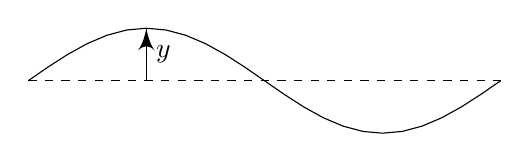
\begin{tikzpicture}
      \draw [domain=0:2] plot ({3*\x}, {sin(\x*180)/1.5});
      \draw [dashed] (0, 0) -- (6, 0);
      \draw [->] (1.5, 0) -- (1.5, 0.666) node [pos = 0.5, right] {$y$};
    \end{tikzpicture}
  \end{center}
  Suppose we pull the line between $x = 0$ and $x = a$ with some tension. Suppose it oscillates with amplitude $y(x; t)$.  Then the kinetic energy is
  \[
    T = \frac{1}{2}\int_0^a \rho v^2\;\d x = \frac{\rho}{2}\int_0^a \dot{y}^2 \;\d x.
  \]
  The potential energy is the tension times the length. So
  \[
    V = T\int \;\d \ell = T\int_0^a\sqrt{1 + (y')^2}\;\d x = (Ta) + \frac{1}{2}T(y'^2)\;\d x.
  \]
  Note that $y'$ is the derivative wrt $x$ while $\dot{y}$ is the derivative wrt time.

  We can ignore that $Ta$ constant, which is the energy initially stored if there is no oscillations, since it doesn't affect where the minimum lies. So the action is
  \[
    S[y] = \int \int_0^a \left(\frac{1}{2}\rho \dot{y}^2 - \frac{1}{2}T(y')^2\right)\;\d x\;\d t
  \]
  We apply the Hamilton's principle which says that we need
  \[
    \delta S[y] = 0.
  \]
  We have
  \[
    \delta S[y] = \int \int_0^a \left(\rho \dot{y} \frac{\partial}{\partial t}\delta y - Ty' \frac{\partial}{\partial x}\delta y\right)\;\d x\;\d t.
  \]
  Integrate by parts to obtain
  \[
    \delta S[y] = \int \int_0^a \delta y(\rho \ddot{y} - Ty'')\;\d x\;\d t + \text{boundary term}.
  \]
  Assuming that the boundary term vanishes, we will need
  \[
    \ddot{y} - v^2 y'' = 0,
  \]
  where $v^2 = T/\rho$. This is the wave equation in two dimensions. Note that this is a linear PDE, which is a simplification resulting from our assuming the oscillation is small.

  Notice that this can be factorized:
  \[
    \left(\frac{\partial}{\partial t} - v\frac{\partial}{\partial x}\right)\left(\frac{\partial}{\partial t} + v\frac{\partial}{\partial x}\right)y(x, t) = 0.
  \]
  So either $\dot y = vy'$ or $\dot y = -vy'$. So we are left with a first-order linear PDE. So
  \[
    y(x, t) = f_+(x - vt) + f_-(x + vt).
  \]
  is the general solution. This is a superposition of a wave travelling rightwards and a wave travelling leftwards.
\end{eg}

\begin{eg}[Maxwell's equations]
  In this case, the kinetic energy is
  \[
    T = \int |\mathbf{E}|^2 + \mathbf{A}\cdot \mathbf{J}\cdot \;\d V.
  \]
  where $\mathbf{E} = -\nabla \phi - \dot{\mathbf{A}}$ is the electric field, $\phi$ is the electric scalar potential, $\mathbf{A}$ is the magnetic vector potential, and $\mathbf{J}$ is the electric current density.

  The potential energy is
  \[
    V = \int (|\mathbf{B}|^2 + \phi \rho)\;\d V,
  \]
  where $\rho$ is the electric charge density, and $\mathbf{B} = \nabla\times \mathbf{A}$ is the magnetic field.

  Then the action is
  \[
    S[\mathbf{A}, \phi] = \int (|\mathbf{E}| - |\mathbf{B}|^2 + \mathbf{A}\cdot \mathbf{J} - \phi \rho)\;\d V\;\d t
  \]
  So
  \[
    \delta S = \int \left(-\mathbf{E}\cdot \left(\nabla \delta\phi + \frac{\partial}{\partial t} \delta \mathbf{A}\right) - \mathbf{B}\cdot \nabla \times \delta \mathbf{A} + \delta \mathbf{A}\cdot \mathbf{J} - \rho\delta\phi\right)\;\d V\;\d t.
  \]
  Integrate by parts to obtain
  \[
    \delta S = \int\delta\left( \mathbf{A}\cdot (\dot{\mathbf{E}} - \nabla\times \mathbf{B} + \mathbf{J}) + \delta \phi(\nabla\cdot \mathbf{E} - \rho)\right)\;\d V\;\d t.
  \]
  Since the coefficients have to be $0$, we must have
  \[
    \nabla \times \mathbf{B} = \mathbf{J} + \dot{\mathbf{E}}.
  \]
  and
  \[
    \nabla \cdot \mathbf{E} = \rho.
  \]
  Also, the definitions of $\mathbf{E}$ and $\mathbf{B}$ give
  \[
    \nabla\cdot \mathbf{B} = 0
  \]
  and 
  \[
    \nabla \times \mathbf{E} = - \dot{\mathbf{B}}.
  \]
  These four equations are Maxwell's equations (in some non-standard units where everything is $1$).
\end{eg}
\section{The second variation}
So far, we have only looked at the ``first derivatives'' of functionals. We can identify stationary points, but we don't know if it is a maximum, minimum or a saddle. So we will have to look at the ``second derivatives'', or the \emph{second variation}.

Suppose $y(x) = y_0(x)$ is a solution of 
\[
  \frac{\delta F[y]}{\delta y(x)} = 0,
\]
, ie. $F[y]$ is stationary at $y = y_0$.

To determine what type of stationary point it is, we need to expand $F[y + \delta y]$ to second order in $\delta y$. For convenience, let $\delta y(x) = \varepsilon \xi(x)$ with $\varepsilon \ll 1$. We will also only consider functionals of the form
\[
  F[y] = \int_\alpha^\beta f(y, y', x)\;\d x
\]
with fixed-end boundary conditions, ie. $\xi(\alpha) = \xi(\beta) = 0$. We expand the integrand to obtain
\begin{align*}
 &f(y + \varepsilon \xi, y' + \varepsilon \xi ', x) - f(y, y', x)\\
 &= \varepsilon \left(\xi \frac{\partial f}{\partial y'} + \xi'\frac{\partial f}{\partial y'}\right)  + \frac{\varepsilon^2}{2}\left(\xi^2 \frac{\partial^2 f}{\partial y^2} + 2\xi\xi' \frac{\partial^2 f}{\partial y \partial y'} + (\xi')^2 \frac{\partial^2 f}{\partial y'^2}\right) + O(\varepsilon^3)\\
 \intertext{Noting that $2\xi \xi' = (\xi^2)'$ and integrating by parts, we obtain}
 &= \varepsilon \xi\left[\frac{\partial f}{\partial y} - \frac{\d}{\d x}\left(\frac{\partial f}{\partial y'}\right)\right] + \frac{\varepsilon^2}{2}\left\{\xi'^2\left[\frac{\partial^2 f}{\partial y^2} - \frac{\d}{\d x}\left(\frac{\partial^2 f}{\partial y\partial y'}\right)\right] + (\xi')^2 \frac{\partial f}{\partial y'^2}\right\}.
\end{align*}
plus some boundary terms which vanish. So
\[
  F[y + \varepsilon \xi] - F[y] = \varepsilon \int_\alpha^\beta\xi\left[\frac{\partial f}{\partial y} - \frac{\d}{\d x}\left(\frac{\partial f}{\partial y'}\right)\right] + \frac{\varepsilon^2}{2}\delta^2 F[y, \xi] + O(\varepsilon^3),
\]
where
\[
  \delta^2 F[y,  \xi] = \int_\alpha^\beta \left\{\xi^2 \left[\frac{\partial^2 f}{\partial y^2} - \frac{\d}{\d x}\left(\frac{\partial^2 f}{\partial y \partial y'}\right)\right] + (\xi')^2 \frac{\partial^2 f}{\partial y'^2}\right\}\;\d x
\]
is a functional of both $y(x)$ and $\xi(x)$. This is analogous to the term
\[
  \delta \mathbf{x}^T H(\mathbf{x})\delta \mathbf{x}
\]
appearing in the expansion of $f(\mathbf{x})$. In the case of normal functions, if $H(\mathbf{x})$ is positive, $f(\mathbf{x})$ is convex for all $\mathbf{x}$, and the stationary point is hence a global minimum. A similar result holds for functionals.

If $\delta^2 F[y, \xi] > 0$ for all non-zero $\xi$ and all allowed $y$, then a solution $y_0(x)$ of $\frac{\delta F}{\delta y} = 0$ is an absolute minimum (where allowed means satisfying boundary conditions plus appropriate smoothness conditions).

\begin{eg}[Geodesics in the plane]
  We previously shown that a straight line is a stationary point for the curve-length functional, but we didn't show it is in fact the shortest distance! Maybe it is a maximum, and we can get the shortest distance by routing to the moon and back.

  Recall that $f = \sqrt{1 + (y')^2}$. Then
  \[
    \frac{\partial f}{\partial y} = 0,\quad \frac{\partial f}{\partial y'} = \frac{y'}{\sqrt{1 + (y')^2}},\quad \frac{\partial^2 f}{\partial y'^2} = \frac{1}{\sqrt{1 + (y')^2}^3},
  \]
  with the other second derivatives zero. So we have
  \[
    \delta ^2 F[y, \xi] = \int_\alpha^\beta \frac{\xi'^2}{(1 + (y')^2)^{3/2}} > 0
  \]
  So if we have a stationary function satisfying the boundary conditions, it is an absolute minimum. Since the straight line is a stationary function, it is indeed the minimum.
\end{eg}
However, not all functions are convex\textsuperscript{[\textcolor{blue}{citation needed}]}. We can still ask whether a solution $y_0(x)$ of the Euler-Lagrange equation is a minimum. For these, we need to consider
\[
  \delta^2 F[y_0, \xi] = \int_\alpha^\beta (\rho(x)(\xi')^2 + \sigma(x) \xi^2)\;\d x,
\]
where
\[
  \rho(x) = \left.\frac{\partial^2 f}{\partial y'^2}\right|_{y = y_0},\quad
  \sigma(x) = \left[\frac{\partial^2 f}{\partial y^2} - \frac{\d}{\d x}\left(\frac{\partial^2 f}{\partial y \partial y'}\right)\right]_{y = y_0}.
\]
This is of the same form as the Sturm-Liouville problem. For $y_0$ to minimize $F[y]$ locally, we need $\delta^2 F[y_0, \xi] > 0$. A necessary condition for this is
\[
  \rho(x) \geq 0,
\]
which is the \emph{Legendre condition}.

The intuition behind this necessary condition is suppose $\rho (x)$ is negative in some interval $I \subseteq [\alpha, \beta]$. Then choose $\xi(x)$ to be zero outside $I$. Inside $I$, we choose it to be small but crazily oscillating. So $\xi'^2$ will be large inside $I$, and so $\delta^2 F[y, \xi]$ can be arbitrarily negative.

However, this is not a sufficient condition. Even if $\rho (x) > 0$ for all $\alpha < x < \beta$, it is still not sufficient.

Of course, a sufficient (but not necessary) condition is $\rho(x) > 0, \sigma(x) \geq 0$.

\begin{eg}
  In the Branchistochrone problem, we have
  \[
    T[y] \propto \int_\alpha^\beta \sqrt{\frac{1 + y'^2}{y}}\;\d x.
  \]
  Then
  \begin{align*}
    \rho(x) &= \left.\frac{\partial^2 f}{\partial y'^2}\right|_{y_0} > 0\\
    \sigma(x) &= \frac{1}{2y^2\sqrt{y(1 + y'^2)}} > 0.
  \end{align*}
  So the cycloid does minimize the time $T$.
\end{eg}
\subsection{Jacobi condition for local minima of \texorpdfstring{$F[y]$}{F[y]}}
For a solution $y_0$ to the Euler Lagrange equation, we have
\[
  \delta^2 F[y_0, \xi] = \int_\alpha^\beta \big(\rho(x) (\xi')^2 + \sigma(x) \xi^2\big)\;\d x,
\]
where
\[
  \rho(x) = \left.\frac{\partial^2 f}{\partial y'^2}\right|_{y = y_0},\quad
  \sigma(x) = \left[\frac{\partial^2 f}{\partial y^2} - \frac{\d}{\d x}\left(\frac{\partial^2 f}{\partial y \partial y'}\right)\right]_{y = y_0}.
\]
Assume $\rho(x) > 0$ for $\alpha < x < \beta$ (the strong Legendre condition) and assume boundary conditions $\xi(\alpha) = \xi(\beta) = 0$. When is this sufficient for $\delta^2 F > 0$? 

First of all, notice that
\[
  0 = \int_\alpha^\beta (w\xi^2)' \;\d x
\]
for any smooth function $w(x)$ since this is a total derivative and evaluates to $w\xi(\alpha) - w\xi(\beta) = 0$. So we have
\[
  0 = \int_\alpha\beta (2w\xi \xi' + w'\xi^2)\;\d x.
\]
This allows us to rewrite $\delta^2 F$ as
\[
  \delta^2 F = \int_\alpha^\beta \big(\rho (\xi')^2 + 2w\xi \xi' + (\sigma + w')\xi^2\big)\;\d x.
\]
Now complete the square in $\xi$ and $\xi'$. So
\[
  \delta^2 F = \int_\alpha^\beta \left[\rho\left(\xi' + \frac{w}{\rho} \xi\right)^2 +\left(\sigma + w' - \frac{w^2}{\rho}\right)\xi^2 \right]
\]
This is $\geq 0$ if
\[
  w^2 = \rho(\sigma + w').\tag{$*$}
\]
We can show that $\delta^2 F$ cannot be zero. If it were, then $\xi' = -\frac{w}{\rho}\xi$. We can solve this to obtain
\[
  \xi(x) = C\exp\left(-\int_\alpha^x \frac{w(s)}{\rho(s)}\;\d s\right).
\]
We know that $\xi(\alpha) = 0$. But $\xi(\alpha) = C e^0$. So $C = 0$. Hence equality holds only for $\xi = 0$.

So $\delta^2 F > 0$ for any allowed non-zero $\xi$ provided we can find a solution of $(*)$. This is a first-order non-linear ODE.

Set $w = --\rho u'/u$. Then $(*)$ becomes
\[
  \rho\left(\frac{u'}{u}\right)^2 = \sigma - \left(\frac{\rho u'}{u}\right) = \sigma - \frac{(\rho u')'}{u} + \rho \left(\frac{u'}{u}\right)^2.
\]
We see that the left and right terms cancel. So we have
\[
  -(\rho u')' + \sigma u = 0.
\]
This is the \emph{Jacobi accessory equation}, a second-order linear ode.

Note that not every solution will do. Within $[\alpha, \beta]$, we cannot have $u = 0$, or else $w = -\rho u'/u$ will be undefined. If we can find a non-zero $u(x)$ satisfying the Jacobi accessory equation, then $\delta^2 F > 0$ for $\xi \not= 0$, and hence $y_0$ is a local minimum of $F$.

In fact, such a solution always exists for sufficiently small $\beta - \alpha$, but may not exist if $\beta - \alpha$ is too large.

% explain intuition.

\begin{eg}[Geodesics on unit sphere]
  For any curve $C$ on the sphere, we have
  \[
    L = \int_C \sqrt{\d \theta^2 + \sin^2 \theta \;\d \phi^2}.
  \]
  If $\theta$ is a good parameter of the curve, then
  \[
    L[\phi] = \int_{\theta _1}^{\theta_2} \sqrt{1 + \sin^2 \theta (\phi')^2}\;\d \theta.
  \]
  Alternatively, if $\phi$ is a good parameter, we have
  \[
    L[\theta] = \int_{\phi_1}^{\phi_2}\sqrt{(\theta')^2 + \sin^2 \theta}\;\d \phi.
  \]
  We will look at the second case.

  We have
  \[
    f(\theta, \theta') = \sqrt{(\theta')^2 + \sin^2 \theta}.
  \]
  So
  \[
    \frac{\partial f}{\partial \theta} = \frac{\sin \theta\cos \theta}{\sqrt{(\theta')^2 + \sin^2 \theta}},\quad \frac{\partial f}{\partial \theta'} = \frac{\theta'}{\sqrt{(\theta')^2 + \sin^2 \theta}}.
  \]
  Since $\frac{\partial f}{\partial \phi} = 0$, we have the first integral
  \[
    \text{const} = f - \theta' \frac{\partial f}{\partial \theta'} = \frac{\sin^2 \theta}{\sqrt{(\theta')^2 + \sin^2 \theta}}
  \]
  So a solution is
  \[
    c\sin^2 \theta = \sqrt{(\theta')^2 + \sin^2 \theta}.
  \]
  Here we need $c \geq 1$ for the equation to make sense.
  
  $c = 1$ happens if $\theta' = 0$. So $\theta$ is constant. Then our first integral gives $\sin^2 \theta = \sin \theta$. So $\sin \theta = 1$ and $\theta = \pi/2$. This is just the equator!

  There are two equatorial solutions to the Euler-Lagrange equations. Which, if any, minimizes $L[\theta]$?
  \begin{center}
    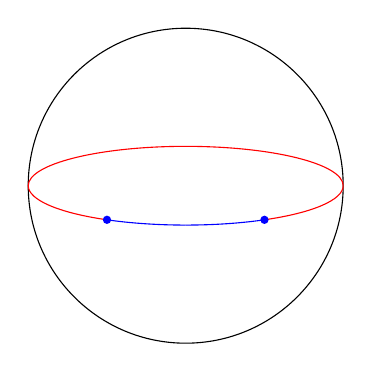
\begin{tikzpicture}
      \draw circle [radius=2];
      \draw [red] (2, 0) arc (0:240:2 and 0.5);
      \draw [red] (2, 0) arc (0:-60:2 and 0.5);
      \draw [blue] (0, -0.5) arc (-90:-60:2 and 0.5) node [circ] {};
      \draw [blue] (0, -0.5) arc (270:240:2 and 0.5) node [circ] {};
    \end{tikzpicture}
  \end{center}
  We have
  \[
    \left.\frac{\partial^2 f}{\partial (\theta')^2}\right|_{\theta = \pi/2} = 1
  \]
  and
  \[
    \frac{\partial^2 f}{\partial \theta \partial \theta'} = -1,\quad \frac{\partial^2}{\partial \theta\partial \theta'} = 0.
  \]
  So $\rho(x) = 1$ and $\sigma(x) = -1$. So
  \[
    \delta^2 F = \int_{\phi_1}^{\phi_2} ((\xi')^2 - \xi^2)\;\d \phi.
  \]
  The Jacobi accessory equation is $u'' + u = 0$. So the general solution is $u \propto \sin \phi - \gamma \cos\phi$. This is equal to zero if $\tan \phi = \gamma$.
  
  Of course, there is always some $\phi_\gamma$ such that $u = 0$. Since $\tan \phi$ is periodic with period $\pi$, we have $u = 0$ for $\phi = \phi_\gamma + n\pi$ for any $\pi$. Hence if our range $\phi_2 - \phi_1$ is greater than $\pi$, it will always contain some values for which $u = 0$. So we cannot conclude that the longer path is a local minimum (it is obviously not a global minimum, by definition of longer) (we also cannot conclude that it is \emph{not} a local minimum, since we tested with a sufficient and not necessary condition).
\end{eg}
\end{document}
